\chapter{Wind Farm Control} \label{sec:ApplicationtoWindFarmControl}

Wind turbines are grouped into farms to efficiently use locations suitable for wind energy harvesting. Within a wind farm, as many turbines as economically viable are installed, with their number limited by wake interactions. A higher turbine density per area reduces the cost of grid connection per turbine and lowers operation and maintenance costs. However, closely spaced turbines experience wake interactions, causing power losses due to reduced energy availability and increased mechanical loads on downstream turbines.
In \cite{houck2022review} wind farm control methods are surveyed, including Axial Induction Control (AIC), Wake Redirection Control (WRC), their combination, and active wake control. These methods have shown advantages in simulations of varying fidelity, and WRC has also demonstrated benefits in field tests. MPC schemes have been proposed in various studies, such as \cite{spudic2014distMPC_https://doi.org/10.1002/oca.2136, zhao2016coordinated, bay2018active, vali2019adjoint}. Unlike individual turbine dynamics, wake interactions in a wind farm cannot be accurately captured by low-order ODEs. Therefore, the approach applied to wind turbine control in Chapter~\ref{sec:Application to Wind Turbine Control4}, i.e., deriving nonlinear differential equations, creating a qLPV model, and using it for qLMPC control, is not applicable to wind farms. But MPC can be utilized by leveraging data-driven models. Recently, Koopman operator-based methods have proven successful \cite{castillo2020wind, cassamo2021model}. By applying Koopman lifting functions to open-loop simulation data and performing Dynamic Mode Decomposition (DMD), state-space models suitable for MPC algorithms can be obtained. AIC strategies have been developed to handle stationary \cite{sharan2022Koopman} and non-stationary inflow conditions \cite{dittmer2022data}, and a combined WRC-AIC scheme has shown potential for tracking high power demands \cite{dittmer2023koopman}.
%
Section \ref{sec:WindFarmSimulationWFSim} revisits the design of WFSim, the wind farm simulation tool used in this thesis, describing the modifications and enhancements necessary to model wind speed variations and to represent thrust and power output for turbines with intentional yaw misalignment. Section \ref{sec:AdaptiveWindFarmqLMPCforAIC} presents an adaptive AIC algorithm capable of handling changes in freestream wind speed. Section \ref{sec:WindFarmLinearMPCforWRC-AIC} first demonstrates wind farm power increases achieved with WRC, followed by a combined WRC-AIC algorithm for grid reference tracking under high power demands. The results of the adaptive AIC scheme have been published in \cite{dittmer2022data}, and those of the combined WRC-AIC algorithm in \cite{dittmer2023koopman}.

\section{Wind Farm Simulation with WFSim} \label{sec:WindFarmSimulationWFSim}
The wind farm simulation environment WFSim \cite{boersma2017tutorial} is employed both for generating open-loop data and for closed-loop controller testing. A short introduction to WFSim is provided in Section~\ref{sec:WakeModels}, which outlines the background on wind farm models and control. The 2D Navier–Stokes equations (NSE) are described in Section~\ref{Subsection:WindFarmSimulationModels}, and the actuator-disk turbine model is introduced in Section~\ref{Subsection:Windfarmcontrol}. WFSim allows the user to either choose from pre-existing layout definitions and sets of control signals, which may be used in open loop, or introduce new sets. A pre-existing layout of a two-turbine farm was selected, but several excitation signal sets were specifically designed for the studies on which this thesis is based as foundations for Koopman system identification. Similar to the easily interchangeable layout and control signal settings, the environment facilitates the integration of custom controller designs. While the flow and pressure calculations are utilized as intended, the applications in this thesis require significant modifications to the internal signal flow of the original MATLAB code.
In its publicly available release, WFSim does not allow variation in wind speed or direction, as the boundary conditions of the 2D wind field are fixed. To overcome this limitation, the code in \cite{dittmer2022data} is adapted to permit time-varying boundary conditions, a prerequisite for demonstrating an adaptive AIC algorithm. Similarly, modifications were introduced in \cite{dittmer2023koopman} to capture more realistic effects of intentional yaw misalignment within the WRC-AIC scheme. By default, the thrust and power coefficients in WFSim are constant. However, since the power coefficient in reality decreases with increasing yaw misalignment \cite{hulsman2022turbine}, the actuator logic was extended with a lookup table. This modification ensures that the controller accurately accounts for the power-loss trade-offs inherent in wake redirection. An overview of the modified program structure, followed by a discussion of the physical concepts represented in the implementation, is provided in the following section. Note that the latter is based on the spatio-temporal discretization and detailed derivation of the 2D NSE found in \cite{boersma2018control}.

\subsection{WFSim Program Structure and Code Modifications} \label{sec:WFSim Program Structure and Code Modifications}
Figure~\ref{fig:WFSimMesh2} illustrates the wind farm layout used for all studies described in this thesis, showing the positions of the two turbines within the simulated wind farm area.
\begin{figure}[htp]
    \centering
    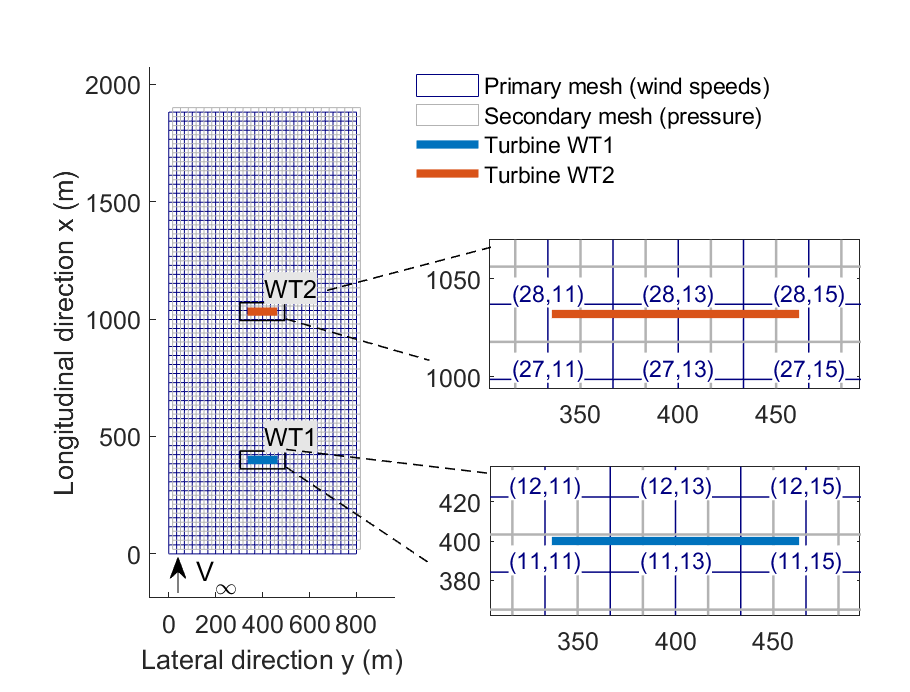
\includegraphics[width=0.65\textwidth]{figures/figures_IFAC23/gridmesh2_tex.eps}
    \caption[WFSim mesh setup for the two-turbine wind farm.]{WFSim mesh setup for the two-turbine wind farm. The primary mesh (blue) is used for wind speed calculations, and the secondary mesh (gray) for pressure. WT1 (upstream) and WT2 (downstream) are shown as blue and red bars, respectively. Zoomed-in areas show primary grid point indices.}
    \label{fig:WFSimMesh2}
\end{figure}
The simulation domain spans~1882\,m in the longitudinal direction and~800\,m in the lateral direction. The primary grid, in blue, is used to compute the longitudinal and lateral wind speeds, and the secondary grid, in gray, is utilized for pressure calculations. Both grids have identical dimensions with a total of 1250 nodes, consisting of 50 nodes in the longitudinal and 25 nodes in the lateral direction. This results in a spatial resolution of $\Delta x = 37.64\,\mathrm{m}$ and $\Delta y = 32\,\mathrm{m}$, with a 1:1 ratio between the primary and secondary grids. The grids are shifted so that the corner nodes of the secondary grid coincide with the center of the mesh cells of the primary grid. The upstream turbine WT1 is represented by a blue bar, and the downstream turbine WT2 by a red bar. The areas around the turbines are shown as zoomed-in plots to clarify which grid points are used in the calculation of the effective wind speeds. For WT1, these are five grid points located in the 11$^{\text{th}}$ row in the longitudinal direction, from the 11$^{\text{th}}$ to the 15$^{\text{th}}$ points in the lateral direction. For WT2, positioned downstream of WT1, the corresponding five points lie in the 27$^{\text{th}}$ longitudinal grid row. 

A considerable speed-up of the WFSim closed-loop simulation is achieved by reformulating the MPC objective function as a QP and avoiding unnecessarily re-initializing constant parameters in each call to the controller. This reformulation of the MPC algorithm results in a speed-up of the controller function execution by a factor of roughly 30 from 152.57\,s to 5.04\,s, and a reduction of the overall simulation time by a factor of nearly 7 from 177.2\,s to 26.2\,s, see Appendix~\ref{appendixC} for further details on the runtimes. Notably, the qLMPC algorithm achieves a mean execution time of 4.2\,ms per simulation step, rendering it potentially real-time capable, whereas the original NMPC requires a mean time of 127.14\,ms. The Koopman MPC algorithms discussed in this thesis are based on this QP formulation of the nonlinear MPC. 

Figure~\ref{fig:WFSimFlow}(a) presents the WFSim program structure diagram for a closed-loop simulation of the original nine-turbine setup. Figure~\ref{fig:WFSimFlow}(b) shows the function used for simulation of Koopman MPC schemes for the two-turbine setup presented in this thesis. While the general program flow and underlying NSE calculations of WFSim are preserved, considerable code modifications and enhancements are necessary in the initialization, the model and the MPC part of the code. These functions are highlighted in Figure~\ref{fig:WFSimFlow}(b) and functions introduced for the Koopman MPC are furthermore written in bold letters. The diagrams are generated using the MATLAB profiler during a closed-loop run with the nonlinear MPC controller integrated into WFSim and the Koopman MPC published in \cite{sharan2022Koopman}. The functions are reordered based on their dependencies to visualize the sequence of function calls.
%\begin{figure}[h]
%    \centering
%    \includegraphics[width=0.65\textwidth, trim=0mm 5mm 7mm 0.1mm, clip]{figuresBlockDiagram_IFAC23/FlowchartInitCtrlPlant_1.eps}
%    \caption{WFSim program structure diagram. Initialization, wind farm model, and controller functions are enclosed in black, blue, and red boxes, respectively. The modified functions \textit{Actuator} and \textit{BoundaryConditions} are highlighted in blue.}
%    \label{fig:WFSimFlow}
%\end{figure}
\begin{figure}[ht]
    \centering
    \subfloat[Original program structure]{
        \begin{minipage}[b]{0.495\textwidth}
            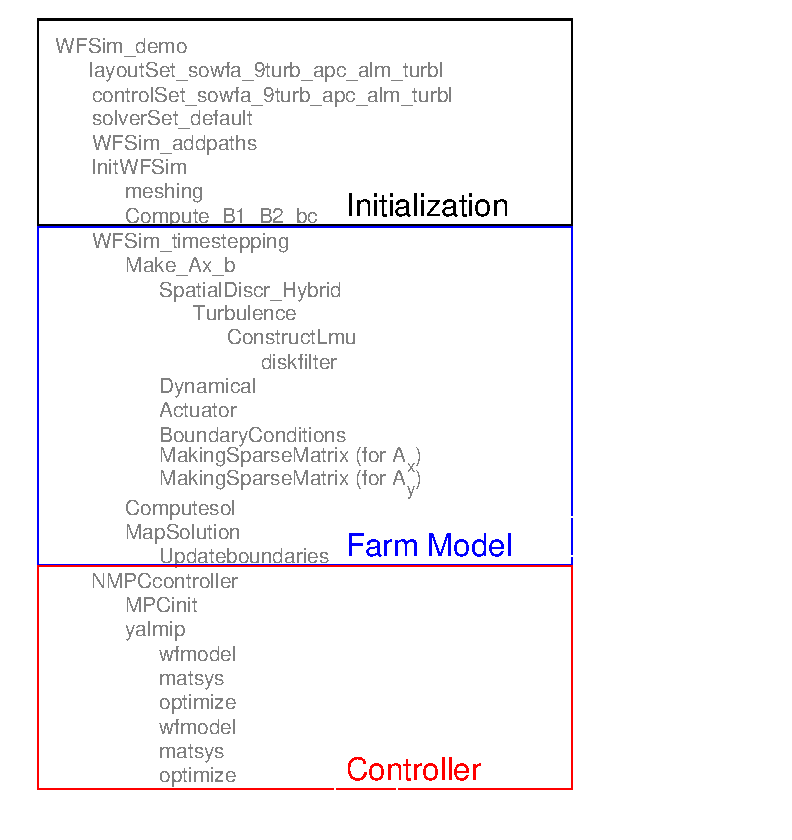
\includegraphics[width=\textwidth, trim=0mm 5mm 29.5mm 0.1mm, clip]{figures/figuresBlockDiagram_IFAC23/FlowchartInitCtrlPlant_1.eps}
        \end{minipage}
    } %\hfill 
    \subfloat[Modified program structure]{
        \begin{minipage}[b]{0.495\textwidth}
            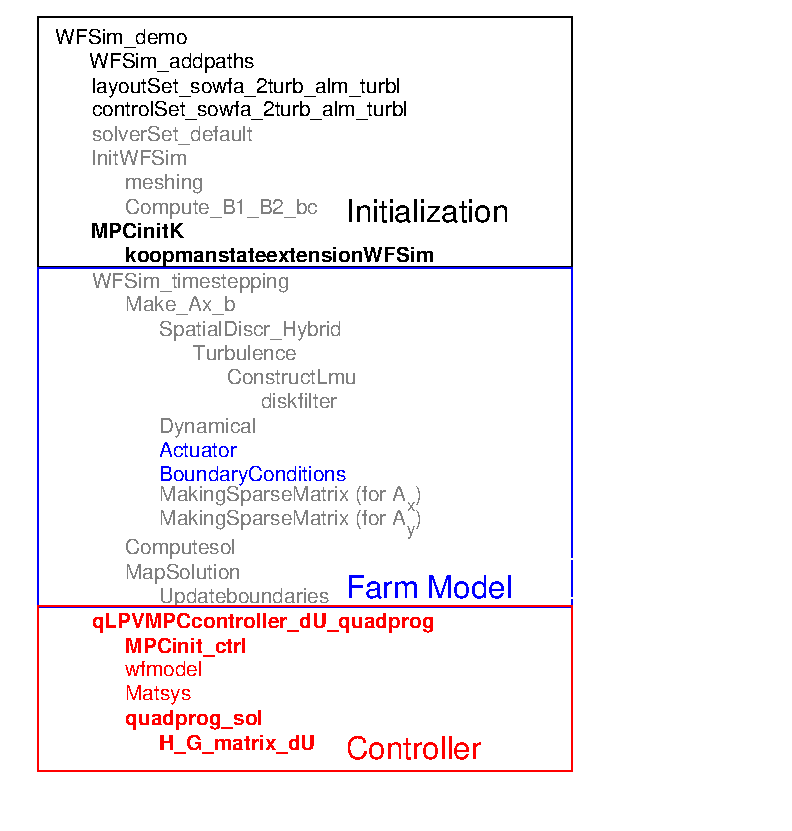
\includegraphics[width=\textwidth, trim=0mm 5mm 29.5mm 0.1mm, clip]{figures/figuresBlockDiagram_IFAC23/FlowchartInitCtrlPlant_2.eps}
        \end{minipage}
    }
    \caption[WFSim program structure diagram.]{WFSim program structure diagram. Initialization, wind farm model, and controller functions are enclosed in black, blue, and red boxes, respectively. Modified functions in (b) are highlighted in black, blue, and red within their respective sections, and functions added for Koopman MPC are indicated in bold.}
    \label{fig:WFSimFlow}
\end{figure}
The entry point to the simulation is the script \textit{WFSim\_demo.m}. Prior to the simulation loop, several initialization functions are called to define the environment and controller parameters as shown in Figure~\ref{fig:WFSimFlow}:

\begin{itemize}\item The script initializes the wind farm layout, setting the number of turbines and their positions, using functions with the naming pattern \textit{layoutSet\_sowfa\_...m}. It specifies the thrust and yaw control signals in \textit{controlSet\_sowfa\_...m}. For the open-loop data generation used to derive the Koopman models presented in \cite{sharan2022Koopman} and \cite{dittmer2022data}, custom signal sets are generated. On the other hand, for closed-loop studies, where only the initial control signal value is selected from the provided vectors and all consecutive control decisions are derived with the control algorithm, the existing files are selected for convenience.
    
    \item The simulation path is set via \textit{WFSim\_addpaths.m} and the solver settings are defined in \textit{solverSet\_default.m}. In the modified structure (Figure~\ref{fig:WFSimFlow}b), the path initialization is the first function to be called, as all commands handling the addition of functions to the executable MATLAB path are moved into this function for a cleaner program structure. It is also modified to ensure that all custom Koopman and QP-based functions can be executed.
    
    \item The function \textit{InitWFSim.m} initializes the wind field, while \textit{meshing.m} defines the computational grid and prepares the MATLAB structures for the simulation.
    
    \item The function \textit{Compute\_B1\_B2\_bc.m} computes the boundary conditions $\bm{b}^\mathrm{BC}$ and the associated matrices $B_1$ and $B_2$. The original implementation calls this function only once, resulting in static boundaries. The modified version calls it whenever the freestream wind changes, enabling non-stationary simulation runs \cite{dittmer2022data}.
    
    \item In the modified program flow, two new functions are added to the initialization phase: \textit{MPCinitK.m} and \textit{koopmanstateextensionWFSim.m}. These functions load the state space model containing the finite-dimensional representation of the Koopman operator, which are used for the subsequent MPC execution.
\end{itemize}
The changes to the turbine states, such as thrust and power, and the wind field at each mesh point are calculated within the simulation loop in \textit{WFSim\_timestepping.m}. The function \textit{Make\_Ax\_b.m} is the core of the WFSim simulation, assembling the system matrices through the following subfunctions:

\begin{itemize}\item In \textit{SpatialDiscr\_Hybrid.m}, a hybrid differencing scheme discretizes the convection terms of the NSE on the 2D mesh. It computes the convection coefficients in both the longitudinal and lateral directions, which are essential for solving the discretized fluid flow equations.
    
    \item The function \textit{Dynamical.m} adds the time-dependent terms of the NSE. It updates the discretization coefficients with unsteady contributions and builds the dynamic source terms representing mass and momentum storage effects based on the velocity field from the previous timestep.
    
    \item The function \textit{Actuator.m} models the actuator-disk representation of the wind turbines within the flow solver. It computes the thrust forces, wake deflection, and power extraction for each turbine. It inserts these forces into the momentum equations and updates turbine data, including power $P$, thrust $F_{T,r}$, yaw $\gamma$, and the coefficients $c_P$ and $c_F$. In \cite{dittmer2023koopman}, a lookup table is integrated into this function to dynamically adjust the power and thrust coefficients based on the yaw angle.
    
    \item In \textit{BoundaryConditions.m}, the boundary conditions for the discretized momentum equations are assigned, enforcing zero-gradient outflow and specific inflow conditions. As shown in the modified structure, this function is adapted in \cite{dittmer2022data} to account for a time-varying freestream wind.
    
    \item The function \textit{MakingSparseMatrix.m} creates the sparse matrix representation of the finite-volume discretization. It is called twice, once for the longitudinal and once for the lateral wind speed components, to construct the system matrices $A_x$ and $A_y$.
\end{itemize}
%
Following the matrix assembly, \textit{Computesol.m} solves the resulting system of equations to obtain the current wind speeds and pressure at the nodes as a vectorized solution. Finally, \textit{MapSolution.m} maps this vector back onto the 2D flow field and updates the boundary conditions for the subsequent simulation iteration. Figure~\ref{fig:WFSimFlow} illustrates the program structure diagram of the controller call within the red box, situated below the wind farm model functions (blue box). In the original code (Figure~\ref{fig:WFSimFlow}a), all controller information, including constant parameters, was re-initialized at every timestep using \textit{MPCinit.m}. In the versions developed in \cite{sharan2022Koopman}, \cite{dittmer2022data}, and \cite{dittmer2023koopman}, only the wind-dependent input matrices are updated, while all constant values are established during the initial setup. In the original implementation, the MATLAB-based modeling framework YALMIP \cite{lofberg2004yalmip} is then initialized to parse the optimization problem. 
%
The thrust commands $C^{\prime}_T$ are calculated in the \textit{NMPCcontroller.m} function through three steps, while the yaw angles $\gamma$ are set to zero:
\begin{itemize}
    \item In \textit{wfmodel.m}, the wind turbine matrices are used to form the wind farm system and input matrices, which are block-diagonal matrices with the turbine matrices on their diagonal.
    \item Based on these, \textit{matsys.m} builds the prediction matrices over the horizon.
    \item The optimal control signals are obtained by solving the resulting MPC problem via the YALMIP function \textit{optimize.m}, with CPLEX as the solver.
\end{itemize}
%
In the modified structure (Figure~\ref{fig:WFSimFlow}b), this workflow is replaced by the \textit{qLPVMPCcontroller\_dU\_\allowbreak quadprog.m} function. This new controller utilizes matrices initialized in \textit{koopmanstateextensionWFSim.m} and initializes wind-dependent input matrices from \textit{MPCinit\_ctrl.m}. The functions \textit{wfmodel.m} and \textit{matsys.m} are modified to accommodate these changes and to construct the parameter-dependent Toeplitz-like matrices and boundary conditions for the QP formulation. These are passed to \textit{quadprog\_sol.m}, which calls the MATLAB solver \textit{quadprog.m}. While the original implementation performed two iterations to refine wind speed predictions, no clear benefit regarding tracking error minimization was observed in the studies forming the basis of this thesis when running the optimization twice. Therefore, the decision was made to calculate the farm control signal only once at each iteration. This further slightly streamlines the process, as less than 3\,ms are now used for each controller calculation. However, it should be noted that this reduction in complexity is secondary to the substantial computational gains achieved by the QP formulation itself.

The following section outlines the calculation of the wind field using the signals $C^{\prime}_T$ and $\gamma$ from \textit{Actuator.m}, the matrices $A_x$ and $A_y$ from \textit{MakingSparseMatrix.m}, and the boundary terms $B_1$, $B_2$, and $\bm{b}^\mathrm{BC}$ from \textit{Compute\_B1\_B2\_bc.m}.

\subsection{Physical Modeling Concepts in WFSim}
In WFSim, wake effects on air pressure and wind speed are modeled using the 2D NSE, which are defined in Equation~\eqref{eq:NSE2d} in Section~\ref{Subsection:WindFarmSimulationModels} and implemented in \textit{Make\_Ax\_b.m} and its subfunctions. For clarity, the NSE are restated here to directly link the physical concepts to their numerical implementation:  
\begin{align*} 
    \frac{\partial \bm{v}}{\partial t}+ (\bm{v}\cdot \nabla_H)\bm{v} + \nabla_H p + \nabla_H\cdot\bm{\tau}_h  - \bm{f} = \bm{0}_{2\times1},\quad  
    \nabla_H\cdot \bm{v} =  -\frac{\partial v_y}{\partial y}
\end{align*}
where $\bm{v} =[v_x\;\;v_y]^T$ consists of the wind components in the $x$- and $y$-directions, respectively. The horizontal gradient operator is $\nabla_H =[\partial/\partial x \;\; \partial/\partial y]^T$, and $p = p(x,y,z_h)$ is the normalized pressure at hub height $z_h$, scaled by air density $\rho_a$. The subgrid stress tensor for horizontal turbulence is denoted by $\bm{\tau}_h$, and $\bm{f}$ represents the turbine-induced forces acting on the flow. These terms are detailed in Section~\ref{Subsection:WindFarmSimulationModels}, which provides the physical background for the wind farm models.

The resulting two-dimensional aerodynamic force vector $\bm{f}_n$, which is applied to the flow field by turbine $n$, is calculated as:
\begin{align}\label{eq:forceNdim2}
    \bm{f}_n =  
    \begin{bmatrix}
        f_{x,n} \\
        f_{y,n}
    \end{bmatrix} 
    = \frac{1}{2} c_f C_{Tn}' \left(V_n \cos(\gamma_n)\right)^2
    \begin{bmatrix}
        \cos(\gamma_n + \phi) \\
        \sin(\gamma_n + \phi)
    \end{bmatrix} \in \mathbb{R}^{2\times 1},
\end{align}
where $C_{Tn}^{\prime}$ is the thrust control signal of turbine $n$ used to regulate axial induction. The variable $\gamma_n$ is the turbine yaw angle, and $\phi$ is the inflow wind direction. The scalar $V_n$ represents the magnitude of the effective wind speed at the rotor center of turbine $n$, and $c_f$ (kg/m) is a model calibration constant used to scale the applied thrust to match high-fidelity simulation or measurement data.

For the numerical implementation, the domain is discretized into an $n_p = n_x \cdot n_y$ grid of pressure cells. WFSim utilizes a staggered grid configuration: the longitudinal wind speed $v_x$ is stored on horizontal cell edges (normal to the vertical x-axis), and the lateral wind speed $v_y$ is stored on the vertical cell edges (normal to the horizontal y-axis). Note that in the WFSim matrix convention, the $x$-axis corresponds to the row index, i.e., the longitudinal direction, and the $y$-axis to the column index, the lateral direction.

This discretization yields $n_{v_x} = n_x \cdot (n_y+1)$ unknowns for the longitudinal velocity and $n_{v_y} = (n_x+1) \cdot n_y$ unknowns for the lateral velocity. Therefore, the 2D force components from Equation~\eqref{eq:forceNdim2} are mapped to the grid and assembled into the vector $\bm{f}$:
\begin{align}\label{eq:forceWFSim}
    \bm{f}_n \;\mapsto\; \bm{f} =
    \begin{bmatrix}
        \bm{f}_{x} \\[1mm]
        \bm{f}_{y}
    \end{bmatrix} \in \mathbb{R}^{(n_{v_x}+n_{v_y}) \times 1}, 
    \qquad 
    \bm{f}_{x} \in \mathbb{R}^{n_{v_x} \times 1}, \quad
    \bm{f}_{y} \in \mathbb{R}^{n_{v_y} \times 1}.
\end{align}
For the example utilized in this thesis, with $n_x = 50$ and $n_y = 25$, the dimensions are:
\begin{align*}
    n_{v_x} = 1300,\;  n_{v_y} = 1275, \;\text{and}\; n_{p} = 1250,
\end{align*}
which results in a total state dimension of $n_q = n_{v_x} + n_{v_y} + n_p = 3825$.

After spatial and temporal discretization, the system dynamics are described by the following differential equation:
\begin{align} \label{eq:WfsinGrid}
    E(q_k)q_{k+1} = Aq_k + \bm{b}(q_k, w_k)
\end{align}
where the system state vector $q_k \in \mathbb{R}^{\,n_q}$ contains the wind speed components and pressure at sample time $k$:
\[
q_k = 
\begin{bmatrix} 
    \bm{v}_x^T   & \bm{v}_y^T   & p^T   
\end{bmatrix}^T \in \mathbb{R}^{\,n_{q} \times 1}.
\]
The control input vector is defined as:
\[
w_k = 
\begin{bmatrix} 
    (\bm{C}_{T,k}^{\prime})^T   & \bm{\gamma}_k^T   
\end{bmatrix}^T   
\in \mathbb{R}^{\,2n_{\mathrm{WT}}\times 1},
\]
where $\bm{C}_{T,k}^{\prime}, \bm{\gamma}_k \in \mathbb{R}^{\,n_{\mathrm{WT}}}$ correspond to the thrust control signals and yaw angles of the $n_{\mathrm{WT}}$ turbines.

The matrices $E(q_k) \in \mathbb{R}^{\,n_{q} \times n_{q}}$ and $A \in \mathbb{R}^{\,n_{q} \times n_{q}}$ describe the interaction between the interior grid points, while $\bm{b}$ is the forcing vector combining boundary conditions and control inputs. Specifically, $E(q_k)$ and  $A$ are structured as
\begin{align} \label{eq:AGrid}
    E(q_k) =
    \begin{bmatrix}
        A_x(\bm{v_{x,k}},\bm{v_{y,k}}) & 0   & B_1 \\
        0   & A_y(\bm{v_{x,k}},\bm{v_{y,k}}) & B_2 \\
        B_1^T   & (2 B_2)^T   & 0
    \end{bmatrix} \text{ and } 
    A =
    \begin{bmatrix}
        A_{11} & 0   & 0 \\
        0   & A_{22} &0 \\
        0   & 0   & 0
    \end{bmatrix},
\end{align}
where $A_x \in \mathbb{R}^{\,n_{v_x} \times n_{v_x}}$ and $A_y \in \mathbb{R}^{\,n_{v_y} \times n_{v_y}}$ are the sparse discretization matrices for the longitudinal and lateral momentum equations.  The matrices $B_1 \in \mathbb{R}^{\,n_{v_x} \times n_p}$ and $B_2 \in \mathbb{R}^{\,n_{v_y} \times n_p}$ couple the pressure field to the momentum equations, while $B_1^T$ and $(2 B_2)^T$ represent the discrete continuity equation acting on the pressure term. The factor of 2 in the $(2B_2)^T$ term arises from a modeling heuristic used to approximate 3D flow effects within a 2D framework. By assuming the vertical flow divergence $\partial w / \partial z$ is approximately equal to the lateral divergence $\partial v / \partial y$, the continuity equation is modified to $\partial u / \partial x + 2\partial v / \partial y = 0$. This adaptation allows the model to simulate mass leakage into the third dimension, preventing the unphysical flow accelerations often seen in standard 2D wake models and providing a better fit to high-fidelity LES data. The diagonal blocks $A_{11} \in \mathbb{R}^{\,n_{v_x} \times n_{v_x}}$ and $A_{22} \in \mathbb{R}^{\,n_{v_y} \times n_{v_y}}$ describe the influence of the longitudinal and lateral velocities at the current time step on those in the next sample.

The forcing vector $\bm{b}(q_k, w_k) \in \mathbb{R}^{n_q\times 1}$ in Equation~\eqref{eq:WfsinGrid} is defined as:
\begin{align} \label{eq:bGrid}\bm{b}(q_k, w_k) =\begin{bmatrix}\bm{f}_x(q_k, w_k) + \bm{b}_x^\mathrm{BC} \\ \bm{f}_y(q_k, w_k) + \bm{b}_y^\mathrm{BC} \\ \bm{0}\end{bmatrix},\end{align}
where $\bm{f}_x$ and $\bm{f}_y$ are the discrete aerodynamic force contributions from the turbines—calculated via the actuator disk model—and $\bm{b}_x^\mathrm{BC}, \bm{b}_y^\mathrm{BC}$ represent the contributions from the velocity boundary conditions. The zero block corresponds to the continuity equation, which remains unforced as it represents the mass conservation constraint. Thus, $\bm{b}(q_k, w_k)$ encompasses all external inputs and boundary constraints driving the state evolution. Although the system state dimension $n_q$ is large, even for the two-turbine case, the matrices are highly sparse and structured due to the finite-volume discretization on the staggered grid. This sparsity allows Equation~\eqref{eq:WfsinGrid} to be solved efficiently using sparse linear algebra techniques.

In the following subsection, the specific wind farm layout and simulation parameters utilized for the studies in this thesis are detailed.
\subsection{WFSim Simulation Setup and Wind Farm Layout}
The simulation studies presented in this thesis, the adaptive AIC \cite{dittmer2022data} and the WRC-AIC \cite{dittmer2023koopman}, utilize an identical wind farm layout. This setup corresponds to the default two-turbine configuration in WFSim, which is also employed in the earlier study \cite{sharan2022Koopman}. The simulation parameters are summarized in Table~\ref{table:WfSim}. 
%
\begin{table}[ht]
    \centering
    \caption{WFSim simulation parameters for the two NREL 5MW turbine setup.}
    \label{table:WfSim}
    \begin{tabular}{l l l l} 
        \toprule
        Description & Symbol & Value & Unit\\
        \midrule
        Domain size &$L_x\times L_y$ & $1882\times 800$& $\text{m}^2$ \\
        Grid size  &$n_x\times n_y$ & $50\times 25$ & -\\
        Number of turbines& $n_{\text{WT}}$ & 2 & - \\
        Rotor diameter & $D$  & $126.4$& m \\
        Turbine spacing & $5D$ & 632 & m\\
        Sample time &$\Delta t$ & $1$ & s \\
        Longitudinal freestream wind &$v_{x,\infty}$&  $7 - 9$ & m/s \\
        Lateral freestream wind &$v_{y,\infty}$  & $0$ & m/s \\         
        Thrust controls & $C^{\prime}_{T,\text{min}}$, $C^{\prime}_{T,\text{max}}$ & 0.1, 2 & -\\
        Yaw angles &$\gamma_1$, $\gamma_2$ &  $0 - 25$, $0$ & deg\\
        \bottomrule
    \end{tabular}
\end{table}
%
The turbines are modeled after the NREL 5MW turbine, featuring a rotor diameter of $D = 126.4\,\text{m}$. They are spaced~$632\,\text{m}$ apart, corresponding to a streamwise distance of five rotor diameters downstream~($5D$). The discrete simulation sample time is set to $1\,\text{s}$. Regarding wind conditions, the lateral freestream component is set to $0\,\text{m/s}$ for both studies. However, the longitudinal freestream wind speed $v_{x,\infty}$ differs: in the adaptive AIC study \cite{dittmer2022data}, it varies between $7\,\text{m/s}$ and $9\,\text{m/s}$, whereas in the WRC-AIC study \cite{dittmer2023koopman}, it is held constant at $8\,\text{m/s}$.

The thrust control inputs $C_T'$ are constrained within the range $[0.1, 2]$.  Both turbines face the wind directly ($\gamma = 0^{\circ}$) in the AIC algorithm. In the WRC-AIC application, the upstream turbine is permitted a maximum yaw misalignment of $25^{\circ}$.

With this simulation setup and the code modifications described in Section~\ref{sec:WFSim Program Structure and Code Modifications}, the adaptive qLMPC algorithm can be applied to the wind farm. The following section discusses the design and implementation of the AIC algorithm.

\section{Adaptive Wind Farm qLMPC with Thrust Control} \label{sec:AdaptiveWindFarmqLMPCforAIC}
Accurately describing the complex turbulence evolution caused by wakes using closed-form low-order ODEs is infeasible. Therefore, the standard MPC controller available in the open-source WFSim environment explicitly models only the turbine dynamics. Wake interactions are accounted for implicitly by utilizing the effective wind speeds at the turbines as inputs to the model. This architecture is illustrated in the block diagram in Figure~\ref{figBlockDiagramFarm}, presented in Section~\ref{Subsection:Windfarmcontrol}, which provides an overview of the WFSim MPC framework.

In this section, the data generation process for both open-loop training and closed-loop controller testing is described. This is followed by a discussion of the data handling procedures required to derive an Extended Dynamic Mode Decomposition (EDMD) model, along with a review of the resulting wind farm model and the MPC algorithm itself. Finally, simulation results for both open-loop wind estimation and closed-loop adaptive control are presented. These results demonstrate the capability of the adaptive algorithm to learn dynamics that were not present in the initial training data.

\subsection{Simulation Setup for Thrust Control}
Figure~\ref{fig:WFSimFlowAIC} visualizes the data flow of the qLMPC scheme for the two-turbine wind farm. The upstream turbine is denoted WT1 and the downstream turbine WT2. A key distinction from the original WFSim implementation is that the effective wind speeds of the turbines are not fed back directly to the controller. Instead, they are estimated using the EDMD-based model introduced in the previous work~\cite{sharan2022Koopman}. While the freestream wind speed was held constant in that study, in this work the longitudinal component $V_\infty = v_{x,\infty}$ is varied, while the lateral component $v_{y,\infty}$ remains zero.

\begin{figure}[htp]
    \centering
    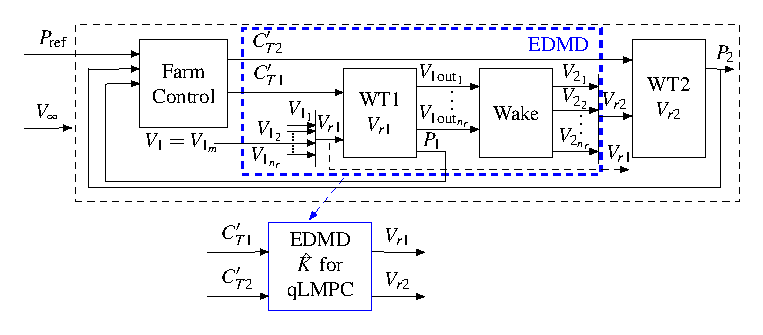
\includegraphics[width=1\textwidth,trim={0 0cm 0cm 0.3cm},clip]{figures/figuresBlockDiagram_IFAC23/farmCtrl16_P_multVthesis_EDMD.pdf}
    \caption[Block diagram of WFSim for AIC]{Block diagram of WFSim for AIC with farm control inputs $P_{\text{ref}}$, $P_1$, $P_2$, and $V_1 = V_{1_m}$, thrust control signals $C_{T1}^{\prime}$ and $C_{T2}^{\prime}$ and freestream wind $V_\infty$. Wind speeds directly in front and behind the turbine WT1 are $V_{1_1}$ to $V_{1_{n_r}}$ and $V_{1\text{out}_1}$ to $V_{1\text{out}_{n_r}}$. Wind speeds directly in front of the turbine WT2 are $V_{2_1}$ to $V_{2_{n_r}}$. The input to the EDMD model (dashed blue box in the closed-loop diagram and blue box below the diagram) are $V_1$, $C_{T1}^{\prime}$ and $C_{T2}^{\prime}$ and its output are the effective wind speeds $V_{r1}$ and $V_{r2}$.}
    \label{fig:WFSimFlowAIC}
\end{figure}

Given that the yaw angle of both turbines is fixed at $0^\circ$ for the AIC algorithm, the effective wind speed calculation, which is defined as the root mean square (RMS) of the wind speeds across the rotor, can be simplified relative to Equation~\eqref{eqEffWindSpdWT} by omitting the cosine term:
\begin{align} \label{eqEffWindSpdWTAIC}
    V_{ri} &=  \sqrt{\frac{1}{n_r} \sum_{j = 1}^{n_r} V_{i_j}^2},  
    \quad  V_{i_j} = v_{x,i_j},
\end{align}
where $v_{x,i_j}$ represents the wind speed component in the $x$-direction at the $j^{\text{th}}$ of $n_r$ mesh points in front of the $i^{\text{th}}$ turbine rotor.

The visualization in Figure~\ref{fig:WFSimFlowAIC} is adapted from the general WFSim diagram (Figure~\ref{figBlockDiagramFarm}) to explicitly distinguish between the local wind speed $V_{1_m}$ and the effective wind speed $V_{r1}$. To achieve this without overcrowding the diagram, the following modifications regarding signals and their visual representation as arrows are made:
\begin{itemize}
    \item In contrast to Figure~\ref{figBlockDiagramFarm}, where local wind speeds were summarized into vectors denoted $\bm{V}_{o1}$ and $\bm{V}_{o2}$, Figure~\ref{fig:WFSimFlowAIC} explicitly displays the individual wind speed signals $V_{1\text{out}_1}$ to $V_{1\text{out}_{n_r}}$ behind WT1. This visualization highlights the spatial signals involved in the wake interaction, while the corresponding signals behind WT2 are omitted, as they do not contribute to the MPC algorithm. Similarly to the rotor outflow, the rotor inflow velocities $V_{1_1}$ to $V_{1_{n_r}}$ and  $V_{2_1}$ to $V_{2_{n_r}}$ are visualized as arrows in Figure~\ref{fig:WFSimFlowAIC}.
    \item The turbine forces resulting from the effective wind speeds and control inputs are calculated within the standard WFSim MPC and are retained as states in the turbine model, see Equation~\eqref{eqPowerWT} in Chapter~\ref{Subsection:Windfarmcontrol} or Equation~\eqref{eqPowerWTAIC_vector}. However, since they are not used in the cost function of either MPC scheme and do not affect the control inputs, they are omitted from Figure~\ref{fig:WFSimFlowAIC} to reduce visual clutter.
\end{itemize}
%
The signals depicted in Figure~\ref{fig:WFSimFlowAIC} are:
\begin{itemize}
    \item Freestream wind $V_\infty$: the freestream wind condition, consisting of a varying longitudinal component $v_{x,\infty}$ and a zero lateral component.
    \item Farm power reference $P_{\text{ref}}$: the reference power output for the entire wind farm.
    \item Wind $V_1$: the local wind speed at the rotor center of the upstream turbine (labeled $V_{1_m}$ in the figure).
    \item Rotor inflow $V_{1_1}$ to $V_{1_{n_r}}$: the array of local wind speeds at the $n_r$ grid points directly in front of the rotor of WT1.
    \item Effective wind $V_{r1}$: the RMS average of the inflow velocities $V_{1_1}$ to $V_{1_{n_r}}$ acting on WT1.
    \item Control signal $C_{T1}^{\prime}$: the thrust control signal applied to WT1.
    \item Power $P_1$: the electrical power generated by WT1.
    \item Rotor outflow $V_{1\text{out}_1}$ to $V_{1\text{out}_{n_r}}$: the local wind speeds at the grid points directly behind WT1.
    \item Rotor inflow $V_{2_1}$ to $V_{2_{n_r}}$: the array of local wind speeds directly in front of the rotor of WT2, which are affected by the wake of WT1.
    \item Effective wind $V_{r2}$: the RMS average of the inflow velocities $V_{2_1}$ to $V_{2_{n_r}}$ acting on WT2.
    \item Control $C_{T2}^{\prime}$: the thrust control signal applied to WT2.
    \item Power $P_2$: the electrical power generated by WT2.
\end{itemize}
Specific signals from this set are recorded during open-loop simulations to construct the linear EDMD models. The identified model utilizes  the thrust control signals $C_{T1}^{\prime}$ and $C_{T2}^{\prime}$, to estimate two outputs, the effective wind speeds $V_{r1}$ and $V_{r2}$.

\subsection{Koopman-Based Identification of qLPV Models}
To derive a Koopman-based linear model for predicting the effective wind speeds, open-loop simulations are first performed to generate training data. Before applying EDMD, this data is lifted using nonlinear functions, following the fundamental principles of Koopman operator theory. This section summarizes the model identification procedure using EDMD and its adaptation for data-driven adaptive control. While the Koopman operator and its matrix representation are described in detail in Sections~\ref{KoopmanOperator} and~\ref{KoopmanIdentification}, key concepts are revisited here to establish the connection to the qLPV model utilized in the wind farm MPC algorithm.

\subsubsection{Koopman Matrix Creation}

Consider a linear system in the lifted space of the form:
\begin{align}
    \bm{\varphi}(k+1) &= \bm{A} \bm{\varphi}(k) + \bm{B} \bm{w}(k), 
    \quad \hat{\bm{x}}(k) = \bm{C} \bm{\varphi}(k), 
    \label{eq:linearPredictor}
\end{align}
where $\bm{\varphi} \in \mathbb{R}^{n_\varphi \times 1}$ is the lifted state vector containing $n_\varphi$ lifted states, and $\bm{w} \in \mathbb{R}^{n_w \times 1}$ denotes the input vector, which may include both control signals and measured disturbances. The vector $\hat{\bm{x}} \in \mathbb{R}^{n_x \times 1}$ represents the predicted output. The system dynamics are defined by the state matrix $\bm{A} \in \mathbb{R}^{n_\varphi \times n_\varphi}$, the input matrix $\bm{B} \in \mathbb{R}^{n_\varphi \times n_w}$, and the output matrix $\bm{C} \in \mathbb{R}^{n_x \times n_\varphi}$. The initial lifted state is given by $\bm{\varphi}(\bm{x}_0) = [g_{1}(\bm{x}_0)\;\; g_{2}(\bm{x}_0) \;\; \ldots\;\;g_{n_\varphi}(\bm{x}_0)]^T$.

In the proposed framework, the lifted state vector $\bm{\varphi}$ is structured such that its first $n_x$ elements correspond directly to the predicted output $\hat{\bm{x}}$, which are the effective wind speeds, followed by their quadratic and cubic terms:
\begin{align*}
    \bm{\varphi} &= [V_{r1} \quad V_{r2} \quad V^2_{r1} \quad V^2_{r2} \quad  V^3_{r1} \quad V^3_{r2}]^T   \in \mathbb{R}^{n_\varphi \times 1}, \\
    \hat{\bm{x}} &=  [V_{r1} \quad V_{r2}] ^T   \in \mathbb{R}^{n_x \times 1},
\end{align*}
with dimensions $n_\varphi = 6$ and $n_x = 2$. The input vector $\bm{w}$ used in this thesis consists of the thrust control signals of the two wind turbines in the wind farm:
\begin{align} \label{eq:wOnlyCt}
    \bm{w} = \bm{u}_{\text{WF}} = [C^{\prime}_{T1} \quad C^{\prime}_{T2}]^T \in \mathbb{R}^{n_w \times 1},
\end{align}
with $n_w = n_u = 2$, as in \cite{sharan2022Koopman}. In \cite{dittmer2022data}, the input vector additionally contained the measured wind speed in front of the upstream turbine. With an improved selection of the identification signals, the models identified without this input reach an acceptable performance level, see the discussion of simulation results in Section~\ref{section:AICWindFarmControl}. This removes the need to measure the freestream wind upstream of the wind farm; the effective wind speeds at the turbines, which initialize the lifted state, are still required. Changes of the freestream wind are then captured by the online model update rather than by a disturbance input.

EDMD is employed to calculate the Koopman matrix, which approximates the infinite-dimensional Koopman operator $\mathcal{K}$ \cite{arbabi2018data}. To facilitate this, the extended lifted states, which combine the nonlinear state lifted states and the inputs, are defined as:
\begin{align}\label{eq:extLiftObs}
    \bm{\varphi}_w(\bm{x},\bm{w}) = 
    \begin{bmatrix}
        \bm{ \varphi}\\ \bm{w}
    \end{bmatrix} \in \mathbb{R}^{(n_\varphi + n_w) \times 1}.
\end{align}
For the considered setup, this results in a total dimension of $n_\varphi + n_w = 9$. Here, $\bm{\varphi} = \bm{g}(\bm{x}) \in \mathbb{R}^{n_\varphi \times 1}$ denotes the vector of nonlinear state lifted states, and $\bm{w} \in \mathbb{R}^{n_w \times 1}$ is the input vector, which appears linearly in the lifted dynamics.

Given $n_o$ samples of state and input data collected in simulation runs, the data snapshot matrices are defined:
\begin{align} \label{eq:DataCollAIC}
    \bm{X} &= \bigl[ [\bm{x}(k)^T \quad \bm{w}(k)^T]^T \bigr]_{k=1}^{n_o-1} \in \mathbb{R}^{(n_x+n_w)\times (n_o-1)}, \\
    \bm{X}_{+} &= \bigl[ [\bm{x}(k+1)^T\quad \bm{w}(k+1)^T]^T \bigr]_{k=1}^{n_o-1} \in \mathbb{R}^{(n_x+n_w)\times (n_o-1)},
\end{align}
where the dimension of the combined state and input vector is $n_x + n_w = 5$. To ensure an accurate approximation of the system dynamics, the number of samples must be significantly larger than the dimension of the extended lifted space ($n_\varphi + n_w$). The data must be sufficiently rich, i.e., excite all relevant frequencies and cover the operating range of interest. For the study presented in \cite{dittmer2022data}, a dataset of $n_o = 32987$ samples, first used in \cite{sharan2022Koopman}, was utilized for identification. While this dataset resulted in satisfying performance for the non-adaptive case at constant wind speed discussed in that earlier study, later investigations showed that for changing wind speeds and an adaptive controller, a newly designed excitation signal exciting a wider range of frequency is beneficial. For the thus slightly modified study presented here, a dataset of $n_o = 29999$ samples is used.

The extended Koopman matrix $\tilde{\bm{K}}$ is obtained by solving the least-squares problem:
\begin{align}
    \min_{\tilde{\bm{K}}} \sum_{k=1}^{n_o-1} 
    \left\|  
    \begin{bmatrix} 
        \bm{g}(\bm{x}(k+1)) \\[1mm] 
        \bm{w}(k+1) 
    \end{bmatrix}   
    - \tilde{\bm{K}} 
    \begin{bmatrix} 
        \bm{g}(\bm{x}(k)) \\[1mm]
        \bm{w}(k) 
    \end{bmatrix} \right\|_2^2.
    \label{eq:ExtendedKoopmanMinimizationProblem}
\end{align}
This matrix possesses the block structure:
\begin{align}
    \tilde{\bm{K}} = \begin{bmatrix} 
        \bm{A}_{\hat{K}} & \bm{B}_{\hat{K}} \\ 
        \bm{A}_{w,\hat{K}} & \bm{B}_{w,\hat{K}} 
    \end{bmatrix},
\end{align}
where 
$\bm{A}_{\hat{K}} \in \mathbb{R}^{n_\varphi \times n_\varphi}$, 
$\bm{B}_{\hat{K}} \in \mathbb{R}^{n_\varphi \times n_w}$, 
$\bm{A}_{w,\hat{K}} \in \mathbb{R}^{n_w \times n_\varphi}$, 
and $\bm{B}_{w,\hat{K}} \in \mathbb{R}^{n_w \times n_w}$.

For controller design, only the system and input matrices $\bm{A}_{\hat{K}}$ and $\bm{B}_{\hat{K}}$ are required. Thus, problem~\eqref{eq:ExtendedKoopmanMinimizationProblem} simplifies to:
\begin{align}
    \min_{\bm{A}_{\hat{K}}, \bm{B}_{\hat{K}}} 
    \sum_{k=1}^{n_o-1} 
    \left\| \bm{g}(\bm{x}(k+1)) - \bm{A}_{\hat{K}} \bm{g}(\bm{x}(k)) - \bm{B}_{\hat{K}} \bm{w}(k) \right\|_2^2.
    \label{eq:ApproxKoopman}
\end{align}
%
With the data matrices defined as
\begin{align}\label{eq:G_Gplus_datamatrices}
    \bm{G} &= \bigl[ \bm{g}(\bm{x}(1)) \;\; \cdots \;\; \bm{g}(\bm{x}(n_o-1)) \bigr] \in \mathbb{R}^{n_\varphi \times (n_o-1)}, \\
    \bm{G}_{+} &= \bigl[ \bm{g}(\bm{x}(2)) \;\; \cdots \;\; \bm{g}(\bm{x}(n_o)) \bigr] \in \mathbb{R}^{n_\varphi \times (n_o-1)}, \\
    \bm{W} &= \bigl[ \bm{w}(1) \;\; \cdots \;\; \bm{w}(n_o-1) \bigr] \in \mathbb{R}^{n_w \times (n_o-1)},
\end{align}
the optimization problem can be equivalently rewritten in matrix form using the Frobenius norm:
\begin{align}
    \min_{\bm{A}_{\hat{K}}, \bm{B}_{\hat{K}}} 
    \left\| \bm{G}_{+} - \bm{A}_{\hat{K}} \bm{G} - \bm{B}_{\hat{K}} \bm{W} \right\|_F^2.
\end{align}
Defining the combined data matrix of lifted states and inputs as:
\begin{align}
    \bm{G}_w = \begin{bmatrix} \bm{G} \\ \bm{W} \end{bmatrix} \in \mathbb{R}^{(n_\varphi + n_w)\times (n_o-1)},
\end{align}
the analytical least-squares solution is given by:
\begin{align}\label{eq:Koop_G_Gplus_datamatrices}
    \hat{\bm{K}} = \begin{bmatrix} \bm{A}_{\hat{K}} & \bm{B}_{\hat{K}} \end{bmatrix} 
    = \bm{G}_{+}  \bm{G}_w^{\dagger}
    \in \mathbb{R}^{n_\varphi \times (n_\varphi + n_w)},
\end{align}
where ${}^\dagger$ denotes the Moore–Penrose pseudoinverse.  The number of samples $n_o$ is typically, as well as in the discussed simulation cases in this thesis, significantly larger than the number of lifted states, i.e., $n_o \gg n_\varphi + n_w$. Provided that the data are sufficiently rich,  $\bm{G}_w$ has full row rank, and the pseudoinverse can be explicitly computed as:
\begin{align*}
    \bm{G}_w^{\dagger} = \bm{G}_w^T (\bm{G}_w \bm{G}_w^T)^{-1} \in \mathbb{R}^{(n_o-1) \times (n_\varphi + n_w)}.
\end{align*}
Substituting this into Equation~\eqref{eq:Koop_G_Gplus_datamatrices} confirms the dimensions:
\[
\underbrace{\hat{\bm{K}}}_{n_\varphi \times (n_\varphi + n_w)} =
\underbrace{\bm{G}_{+}}_{n_\varphi \times (n_o-1)} \cdot
\underbrace{\bm{G}_w^T}_{(n_o-1) \times (n_\varphi + n_w)} \cdot
\underbrace{(\bm{G}_w \bm{G}_w^T)^{-1}}_{(n_\varphi + n_w) \times (n_\varphi + n_w)}.
\]
Equivalently, the identified matrix can be written as $\hat{\bm{K}}_0 = \mathbf{L}_0\,\mathbf{L}_{u,0}^{-1}$ with the initial auto- and cross-correlation matrices
\begin{align*}
    \mathbf{L}_{u,0} = \bm{G}_w \bm{G}_w^T, \quad \mathbf{L}_0 = \bm{G}_{+} \bm{G}_w^T,
\end{align*}
which serve as initial values for the online update explained below.
%
To utilize the identified matrix $\hat{\bm{K}}$ for linear model predictive control, it is partitioned into the system matrix $\bm{A}_{\hat{K}} \in \mathbb{R}^{n_\varphi \times n_\varphi}$ and the input matrix $\bm{B}_{\hat{K}} \in \mathbb{R}^{n_\varphi \times n_w}$. The system matrix consist of the first $n_\varphi$ columns of $\hat{\bm{K}}$, the input matrix of the remaining  $n_w$ columns, see Equation~\eqref{eq:Koop_G_Gplus_datamatrices}.

In \cite{dittmer2022data}, the measured disturbance $V_1$ is part of the input vector, i.e., $n_w = 3$, and needs to be accounted for as an autonomous state within the prediction horizon. In this case, the input matrix is further split into $\bm{B}_{\hat{K},d} \in \mathbb{R}^{n_\varphi \times n_d}$ for the $n_d$ disturbances and $\bm{B}_{\hat{K},u} \in \mathbb{R}^{n_\varphi \times (n_w-n_d)}$ for the control inputs $[C'_{T1} \;\; C'_{T2}]^T$. The final augmented Koopman matrix $\hat{\bm{K}}_{\text{aug}}$ is then constructed to include the disturbance dynamics. Assuming the disturbance remains constant over the prediction horizon, the augmentation is performed as follows:
\begin{align}\label{eq:AugmentedKoopmanMPC}
    \hat{\bm{K}}_{\text{aug}} = \left[\begin{array}{cc|c}
        \bm{A}_{\hat{K}} & \bm{B}_{\hat{K},d} & \bm{B}_{\hat{K},u}\\
        \bm{0}_{n_d \times n_\varphi} & \bm{I}_{n_d} & \bm{0}_{n_d \times (n_w-n_d)}
    \end{array}\right] \in \mathbb{R}^{(n_\varphi+n_d) \times (n_\varphi+n_w)},
\end{align}
where the second block row ensures the persistence of the measured wind speed disturbance throughout the prediction, with $n_d = 1$ in this case. This structure allows the MPC to treat the disturbance as a known, constant state during the optimization of the control sequence. If the vector $\bm{w}$ consists only of control inputs, see Equation~\eqref{eq:wOnlyCt}, then $n_d = 0$ and hence $\hat{\bm{K}}_{\text{aug}} = \hat{\bm{K}}$.


\subsubsection{Koopman Matrix Update}\label{subsec:koopmanOnlineUpdate}

The online update strategy employed here is based on the recursive least squares method proposed in \cite{cisneros2020data}. To minimize computational overhead and memory usage, the model is not updated continuously. Instead, an update is triggered only when the deviation between the measured outputs and the model predictions over a window of length $h$ exceeds a defined threshold $\nu$.

Let $\mathcal{X}_{\nu}$ denote the buffer containing the state and input vectors from the previous $h+1$ time instants:
\[
\mathcal{X}_{\nu} = \begin{bmatrix} x_{k-1}^T & w_{k-1}^T & \dots & x_{k-h-1}^T & w_{k-h-1}^T \end{bmatrix} \in \mathbb{R}^{1 \times (n_x + n_w)(h+1)}.
\]
The triggering condition is formulated using the infinity norm, which allows the threshold $\nu$ to be interpreted in physical units independent of the window length $h$:
\begin{equation} \label{eq:add_data}
    \left\|
    \begin{bmatrix}
        x_{k-h} \\
        x_{k-h+1} \\
        \vdots \\
        x_{k}
    \end{bmatrix}
    -
    \begin{bmatrix}
        C\hat{K}\bm{\varphi}_w(z_{k-h-1}) \\[2mm]
        C\hat{K}\bm{\varphi}_w\Big(
        \begin{bmatrix}
            \hat{K}\bm{\varphi}_w(z_{k-h-1}) \\
            w_{k-h}
        \end{bmatrix}
        \Big) \\[1mm]
        \vdots \\[1mm]
        C\hat{K}\bm{\varphi}_w\Big(
        \begin{bmatrix}
            \hat{K}\bm{\varphi}_w\Big(
            \begin{bmatrix}
                \hat{K}\bm{\varphi}_w(\cdots) \\
                w_{k-2}
            \end{bmatrix}
            \Big) \\
            w_{k-1}
        \end{bmatrix}
        \Big)
    \end{bmatrix}
    \right\|_\infty \geq \nu,
\end{equation}
where the extended lifted lifted states $\bm{\varphi}_w$ are defined as in Equation~\eqref{eq:extLiftObs}, and $z_k = [x_k^T \;\; w_k^T]^T$ is a stacked vector selected from $\mathcal{X}_{\nu}$.

When this condition is met, the Koopman matrix is updated using the data matrices $\mathbf{L}_u^+$ and $\mathbf{L}^+$. At initialization, $\mathbf{L}_u$ and $\mathbf{L}$ are the offline correlation matrices defined above. While \cite{cisneros2020data} utilizes only the current measurement, this work incorporates a batch of the last five measurement samples to provide low-pass filtering and reduced sensitivity to noise. The batch data matrices are defined as
\[
z_{k,5} = [z_{k-5} \;\; z_{k-4} \;\; \dots \;\; z_{k-1}] \in \mathbb{R}^{(n_x + n_w)\times 5}, \quad
x_{k,5}^+ = [x_{k-4} \;\; x_{k-3} \;\; \dots \;\; x_{k}] \in \mathbb{R}^{n_x \times 5},
\]
where $x_{k,5}^+$ contains the successor states of the samples in $z_{k,5}$.
The recursive updates are computed as a weighted sum of the existing correlation matrices $\mathbf{L}_u$ and $\mathbf{L}$ and the new data:
\begin{equation} \label{eq:GA_online}
    \begin{split}
        n_{\text{upd}}^+ &= n_{\text{upd}} + 1,\\
        \mathbf{L}_u^+ &= \frac{1}{n_{\text{upd}}^+} \Big( (n_{\text{upd}}^+-1)\mathbf{L}_u + \bm{\varphi}_w(z_{k,5}) \bm{\varphi}_w(z_{k,5})^T \Big),\\
        \mathbf{L}^+ &= \frac{1}{n_{\text{upd}}^+} \Big( (n_{\text{upd}}^+-1)\mathbf{L} + \bm{\varphi}(x_{k,5}^+) \bm{\varphi}_w(z_{k,5})^T \Big).
    \end{split}
\end{equation}
The updated Koopman matrix is then obtained as $\hat{\bm{K}}^+ = \mathbf{L}^+ (\mathbf{L}_u^+)^{-1}$ and partitioned as in Equation~\eqref{eq:Koop_G_Gplus_datamatrices}. In \cite{dittmer2022data}, this is the augmented Koopman matrix which is split up according to Equation~\eqref{eq:AugmentedKoopmanMPC}.
The counter $n_{\text{upd}}$ acts as a weighting factor. In \cite{cisneros2020data}, this counter monotonically increases. In contrast, here the counter $n_{\text{upd}}$ is reset to $1$ whenever the error norm falls below the threshold. This allows the model to adapt to changing dynamics rather than becoming rigid due to a large historical weight. During active updates, the counter is incremented to integrate the new information.

Finally, accurate online identification requires sufficient spectral content in the input. Since standard control signals may not excite all dynamic modes, a low-amplitude band-limited white noise signal is superimposed on the control input during updates.
%More details on the implementation of this excitation signal are provided in the results section.
%Future improvements may include explicit limits on $n_{\text{upd}}$ and the introduction of forgetting factors to balance recent and historical data, as suggested in \cite{zhang2019online}.
%Based on the theory in \cite{cisneros2020data}, a brief review on online update of koopman model is provided in this section. To avoid the memory management issues, we can only store $G$, $G_+$ and $U$ vectors at time $k$ ToDo: Make clear that Psi might be a matrix not a vector if more than one sample is included. Aso use our formulation  Phi*Phi' and X1 *Phi' where Phi= [x0;u0] 
% To do: Forgetting factors, weights between previous model and new data, 
% 'keep alert', find balance between new information
% add quotes (Zhang, Princeton, adaptive DMD) ,added several samples
% Differences to Pable: P initialized as 1, so offline identified model is used
% P is reset to 1 when no update is necessary (tuning knob -> future work to 
\subsection{qLMPC Design for Thrust Control} 
The aim of wind farm control considered here is accurate tracking of a power reference with minimal changes in the control inputs, as discussed, e.g., in \cite{vali2019adjoint, boersma2019constrained}.
\subsubsection{Model Derivation and Cost Function}
As mentioned in Section~\ref{Subsection:Windfarmcontrol}, the main difference to the NMPC that ships with WFSim is that the effective wind speeds over the prediction horizon are predicted with a data-driven Koopman model instead of being kept constant. This turns the wind farm model into a qLPV model, as its input matrices depend on the predicted effective wind speeds. The Koopman model is identified with EDMD from data acquired in open-loop WFSim simulations. It uses the wind speed in front of the first turbine $V_1$ and the two thrust control signals $C_{T1}^{\prime}$ and $C_{T2}^{\prime}$ as inputs and the resulting effective wind speeds as states. Before applying EDMD, the data is extended with nonlinear lifting functions, following the Koopman approach discussed in detail in Section~\ref{KoopmanIdentification}.

For the qLMPC design for adaptive AIC, the same discrete-time wind farm model is used as in the original WFSim NMPC algorithm described in Section~\ref{Subsection:Windfarmcontrol} in Equations~\eqref{eqPowerWT} to~\eqref{eqLinWF}. The procedure used to calculate the evolution of the wind farm power over a prediction horizon is repeated here for ease of understanding, with the only difference being that the yaw angle is fixed to zero. The state-space model of the $i^{\text{th}}$ turbine, assuming no yaw control or misalignment, is given by:
\begin{align} \label{eqPowerWTAIC_vector}
    \underbrace{
        \begin{bmatrix}
            P_i(k+1) \\[0.8mm]
            F_{T,ri}(k+1) \\[0.8mm]
            \hat{C}_{Ti}^\prime(k+1)
    \end{bmatrix}}_{\bm{x}_{\text{WT},i}(k+1) \in {\mathbb{R}}^{3\times 1}}
    &=
    \underbrace{(1-\tau)\,\bm{I}_{3\times3}}_{\bm{A}_{\text{WT},i} \in {\mathbb{R}}^{3\times 3}}
    \begin{bmatrix}
        P_i(k) \\[0.8mm]
        F_{T,ri}(k) \\[0.8mm]
        \hat{C}_{Ti}^\prime(k)
    \end{bmatrix}
    +
    \underbrace{\tau
        \begin{bmatrix}
            \tfrac{1}{2}\rho_a A_r \hat{V}_{ri}^3 \\[0.8mm]
            \tfrac{1}{2}\rho_a A_r \hat{V}_{ri}^2 \\[0.8mm]
            1
    \end{bmatrix}}_{\bm{B}_{\text{WT},i}(\hat{V}_{ri}) \in {\mathbb{R}}^{3\times 1}} \, C_{Ti}^\prime(k),
\end{align}
where $k$ is the discrete sample time index and the constant $\tau$ is the discrete-time filter coefficient. The coefficient $\tau$ determines the weighting between the current state and the new input at each time step, thereby controlling the response speed of the turbine states. In contrast to the original WFSim NMPC, the input matrix depends on the predicted effective wind speed $\hat{V}_{ri}$.

In the state vector $\bm{x}_{\text{WT},i}$, $P_i$ denotes the power, $F_{T,ri}$ the thrust force of the $i$-th turbine, and $\hat{C}_{Ti}^\prime$ the filtered thrust control signal:
\begin{align*}
    \bm{x}_{\text{WT},i} = [P_i \quad F_{T,ri} \quad \hat{C}_{Ti}^\prime]^T.
\end{align*}
The thrust force $F_{T,ri}$ is retained in the state vector to remain consistent with the original WFSim implementation, in which it is computed as part of the turbine model. Since $\bm{A}_{\text{WT},i}$ is diagonal, $F_{T,ri}$ does not influence the other states, and it is not penalized in the cost function. It therefore has no effect on the control inputs computed by the MPC.

The individual turbine models are concatenated into a qLPV system with the vector of all predicted effective wind speeds $\hat{\bm{V}}_r$ as the scheduling parameter vector:
\begin{align} \label{eqLinWFAIC}
    \bm{x}_{\text{WF}}(k+1) &= \bm{A}_{\text{WF}} \bm{x}_{\text{WF}}(k) + \bm{B}_{\text{WF}}(\hat{\bm{V}}_r(k)) \, \bm{C}_{T}^\prime(k),\\
    P_{\text{WF}}(k) & = \underbrace{\bm{1}_{1 \times n_{\text{WT}} } \otimes [1 \quad 0 \quad 0]}_{\bm{C}_{\text{WF}} \in {\mathbb{R}}^{1 \times 3n_\text{WT}}} \, \bm{x}_{\text{WF}}(k), \label{eqLinWFAIC2}
\end{align}
where $\bm{A}_{\text{WF}} \in {\mathbb{R}}^{3n_\text{WT} \times 3n_\text{WT}}$ and $\bm{B}_{\text{WF}}(\hat{\bm{V}}_r) \in {\mathbb{R}}^{3n_\text{WT} \times n_\text{WT}}$ are block-diagonal matrices composed of the turbine matrices $\bm{A}_{\text{WT},i}$ and $\bm{B}_{\text{WT},i}(\hat{V}_{ri})$. The wind farm power $P_{\text{WF}}$ is the sum of all individual turbine powers, $P_{\text{WF}} = \sum_{i=1}^{n_{\text{WT}}} P_i$.

The farm-level state vector, the control input vector, and the vector containing the estimated effective wind speeds of all turbines are defined as:
\begin{align*}
    \bm{x}_{\text{WF}} &= [\bm{x}_{\text{WT},1}^T \quad \bm{x}_{\text{WT},2}^T \quad \dots \quad \bm{x}_{\text{WT},n_{\text{WT}}}^T ]^T \in {\mathbb{R}}^{3n_\text{WT} \times 1},\\
    \bm{C}_{T}^\prime &= [C_{T1}^\prime \quad C_{T2}^\prime \quad \dots \quad C_{T n_{\text{WT}}}^\prime ]^T \in {\mathbb{R}}^{n_\text{WT} \times 1},\\
    \hat{\bm{V}}_r &= [\hat{V}_{r1} \quad \hat{V}_{r2} \quad \dots \quad \hat{V}_{r n_\text{WT}}]^T \in {\mathbb{R}}^{n_\text{WT}\times 1}.
\end{align*}
The vector $\hat{\bm{V}}_r$ is the scheduling parameter vector $\bm{\rho}_{\Rho,\text{WF}}$ introduced in Equation~\eqref{eq:rhoWF}. Over the prediction horizon, it forms the scheduling trajectory
\begin{align*}
    \bm{\Rho}_{\Rho} = [ \hat{\bm{V}}_r^T(k) \quad \hat{\bm{V}}_r^T(k+1) \quad \ldots \quad \hat{\bm{V}}_r^T(k+n_h-1)]^T \in \mathbb{R}^{n_{\text{WT}} n_h \times 1}.
\end{align*}
%
These vectors are used in combination with the parameter-dependent Toeplitz-like matrices built from $\bm{A}_{\text{WF}}$, $\bm{B}_{\text{WF}}$, and $\bm{C}_{\text{WF}}$ to predict the farm power trajectory, similarly to the approach discussed in Section~\ref{sec:qLMPCOptimizationAlgo} and Equation~\eqref{eq:nearlyToeplitzMat}.
% \bm{\varphi}_w
The cost function $J(\bm{U})$ is formulated to minimize the tracking error $\bm{E}$ and control increments $\Delta \bm{U}$:
\begin{align} \label{eq:NMPCcostAIC}
    J(\bm{U}) = \underbrace{\bm{E}^T Q \bm{E}}_{J_Q (\bm{U})} + \underbrace{\Delta \bm{U}^T R \Delta \bm{U} }_{J_R ( \bm{U})},
\end{align}
with weighting matrices $Q = q \cdot \bm{I}_{n_h \times n_h}$ and $R = r \cdot \bm{I}_{n_{hu}\times n_{hu}}$. The tracking error trajectory $\bm{E}(k)$ is defined as:
\begin{equation}\label{eq:errortraject}
    \begin{aligned}
        \bm{E}(k) &= \bm{P}_{\text{ref}}(k) - \hat{\bm{P}}_{\text{WF}}(k) \\
        &= [ e(k+1) \quad e(k+2) \quad \dots \quad e(k + n_h) ]^T \in \mathbb{R}^{n_h \times 1},
    \end{aligned}
\end{equation}
where $e = P_{\text{ref}} - \hat{P}_{\text{WF}}$, i.e., the difference between the reference farm-level power $P_{\text{ref}}$ and the predicted power $\hat{P}_{\text{WF}}$. The reference, predicted power, and control trajectories are given by:
\begin{equation} \label{eq:UandDUAIC}
    \begin{aligned}
        \bm{P}_{\text{ref}}(k) &= [ P_{\text{ref}}(k+1) \quad P_{\text{ref}}(k+2) \quad \dots \quad P_{\text{ref}}(k + n_h)]^T \in \mathbb{R}^{n_h \times 1}, \\
        \hat{\bm{P}}_{\text{WF}}(k) &= [ \hat{P}_{\text{WF}}(k+1) \quad \hat{P}_{\text{WF}}(k+2) \quad \dots \quad \hat{P}_{\text{WF}}(k + n_h)]^T \in \mathbb{R}^{n_h \times 1}, \\
        \bm{U}(k) &= [ \bm{C}_T^{\prime T}(k) \quad \bm{C}_T^{\prime T}(k+1) \quad \dots \quad \bm{C}_T^{\prime T}(k+n_h-1) ]^T \in \mathbb{R}^{n_{hu}\times 1},
    \end{aligned}
\end{equation}
with the length of the control trajectory $n_{hu} = n_h n_{\text{WT}}$, as each turbine has a single control input, its thrust coefficient $C'_{Ti}$. The first element $\bm{C}_T^\prime(k)$ of $\bm{U}(k)$ is the input applied at the current sample, which affects the power from sample $k+1$ onward. The reference trajectory $\bm{P}_{\text{ref}}(k)$ is assumed to be known over the prediction horizon. The trajectory of the control increments contains the changes of the thrust control vector between consecutive time steps:
\begin{align} \label{eq:DUAIC}
    \Delta \bm{U}(k) = [ \Delta\bm{C}_T^{\prime T}(k) \quad \Delta\bm{C}_T^{\prime T}(k+1) \quad \dots \quad \Delta\bm{C}_T^{\prime T}(k+n_h-1) ]^T \in \mathbb{R}^{n_{hu}\times 1},
\end{align}
with $\Delta\bm{C}_T^\prime(k) = \bm{C}_T^\prime(k) - \bm{C}_T^\prime(k-1)$, where $\bm{C}_T^\prime(k-1)$ is the input applied at the previous sample. For the two-turbine case with $n_h = 10$, this yields $\bm{E} \in \mathbb{R}^{10\times 1}$ and $\bm{U}, \Delta \bm{U} \in \mathbb{R}^{20\times 1}$. Finally, the constrained optimization problem is stated as:
\begin{align} \label{eq:ObjFunAIC}
    \begin{array}{ll}
        \underset{\bm{U}(k)}{\text{minimize }} & J(\bm{U}(k)) = \bm{E}^T(k) Q \bm{E}(k) + \Delta \bm{U}^T(k) R \Delta \bm{U}(k) = J_Q(\bm{U}) + J_R(\bm{U}) \\[10pt]
        \text{subject to} & \bm{x}_{\text{WF}}(k+j+1) = \bm{A}_{\text{WF}} \bm{x}_{\text{WF}}(k+j) + \bm{B}_{\text{WF}}(\hat{\bm{V}}_r(k+j)) \bm{C}_{T}^\prime(k+j), \\[10pt]
        & \hat{P}_{\text{WF}}(k+j+1) = \bm{C}_{\text{WF}} \bm{x}_{\text{WF}}(k+j+1), \\[10pt]
        & \bm{C}_{T,\text{min}}^\prime \leq \bm{C}_{T}^\prime(k+j) \leq \bm{C}_{T,\text{max}}^\prime, \quad j = 0, \dots, n_h-1,
    \end{array}
\end{align}
with the current turbine states $\bm{x}_{\text{WF}}(k)$ as initial condition and the limits $\bm{C}_{T,\text{min}}^\prime$ and $\bm{C}_{T,\text{max}}^\prime$ of the thrust control signals.

\subsubsection{Power Prediction, Control Increments and Cost Terms for QP Formulation}
Note that the decision variables in the wind farm optimization problem in Equation~\eqref{eq:ObjFunAIC} are the elements of $\bm{U}$, not of $\Delta \bm{U}$. This is a difference to the velocity-based wind turbine qLMPC in Equation~\eqref{eq:ObjFunWT}. There, the underlying state-space model is velocity-based, so both the error term $\bm{e}$ and the control term depend directly on the decision variable increment $\Delta\bm{u}_{\text{Mdl}^\prime}$. Here, for wind farm control, the error term $\bm{E}$ depends on $\bm{U}$, while the control term depends on $\Delta\bm{U}$. To obtain a QP in $\bm{U}$, both terms are therefore expressed in terms of $\bm{U}$, as shown in the following.

The predicted power trajectory follows from the state-space model in Equation~\eqref{eqLinWFAIC}:
\begin{align*}
    %\hat{\bm{P}}_{\text{WF}}(k) = \tilde{L}\, \bm{x}_{\text{WF}}(k) + \tilde{S}(\hat{\bm{V}}_r)\, \bm{U}(k),
    \hat{\bm{P}}_{\text{WF}}(k) = \tilde{L}\, \bm{x}_{\text{WF}}(k) + \tilde{S}(\bm{\Rho}_k)\, \bm{U}(k),
\end{align*}
with the matrices $\tilde{L} \in \mathbb{R}^{n_h \times 3n_{\text{WT}}}$ and $\tilde{S} \in \mathbb{R}^{n_h \times n_{hu}}$:
\begin{equation} \label{eq:ltildeWF}
    \begin{aligned}
        \tilde{L} &=
        \begin{bmatrix}
            \bm{C}_{\text{WF}} \bm{A}_{\text{WF}} \\ \bm{C}_{\text{WF}} \bm{A}_{\text{WF}}^2 \\ \vdots \\ \bm{C}_{\text{WF}} \bm{A}_{\text{WF}}^{n_h}
        \end{bmatrix}, \\
        \tilde{S}(\hat{\bm{V}}_r) &=
        \begin{bmatrix}
            \bm{C}_{\text{WF}} \bm{B}_{\text{WF},0} & \bm{0} & \cdots & \bm{0} \\
            \bm{C}_{\text{WF}} \bm{A}_{\text{WF}} \bm{B}_{\text{WF},0} & \bm{C}_{\text{WF}} \bm{B}_{\text{WF},1} & \cdots & \bm{0} \\
            \vdots & \vdots & \ddots & \vdots \\
            \bm{C}_{\text{WF}} \bm{A}_{\text{WF}}^{n_h-1} \bm{B}_{\text{WF},0} & \bm{C}_{\text{WF}} \bm{A}_{\text{WF}}^{n_h-2} \bm{B}_{\text{WF},1} & \cdots & \bm{C}_{\text{WF}} \bm{B}_{\text{WF},n_h-1}
        \end{bmatrix},
    \end{aligned}
\end{equation}
where $\bm{B}_{\text{WF},j} = \bm{B}_{\text{WF}}(\hat{\bm{V}}_r(k+j))$ is the input matrix evaluated with the predicted effective wind speeds at step $k+j$. Only $\tilde{S}$ depends on the predicted wind speeds, since $\bm{A}_{\text{WF}}$ and $\bm{C}_{\text{WF}}$ are constant. The current state $\bm{x}_{\text{WF}}(k)$ initializes the prediction and is calculated from the state and input at the previous sample $k-1$.

To evaluate the qLPV wind farm model over the prediction horizon, the effective wind speeds $\hat{V}_{ri}(k+j)$, $j = 1, \dots, n_h$, are required. In \cite{dittmer2022data}, they are predicted with the identified Koopman model in its augmented form, see Equation~\eqref{eq:AugmentedKoopmanMPC}. The prediction starts from the lifted state $\hat{\bm{\varphi}}(k)$ predicted at the previous time step. The inputs, i.e., the thrust coefficients $\bm{C}_T^\prime(k-1)$ applied at the previous sample and, formerly, the measured upstream wind speed $V_1(k)$, are held constant over the horizon. As the matrices $\bm{A}_{\hat{K}}$ and $\bm{B}_{\hat{K}}$ are identified without the wind input and from different open-loop data, they differ from those of \cite{dittmer2022data}. With no wind measurement for the prediction of the effective wind speeds and with matrices $\bm{A}_{\hat{K}}$ and $\bm{B}_{\hat{K}}$ as defined in Equation~\eqref{eq:Koop_G_Gplus_datamatrices} the lifted state trajectories are:
\begin{align*}
    \hat{\bm{\varphi}}(k+j) &= \bm{A}_{\hat{K}}\, \hat{\bm{\varphi}}(k+j-1) + \underbrace{\bm{B}_{\hat{K},u}}_{\bm{B}_{\hat{K}}}\, \bm{C}_T^\prime(k-1) + \cancel{\bm{B}_{\hat{K},d}\, V_1(k)}, \\
    \hat{\bm{V}}_r(k+j) &= \bm{C}\, \hat{\bm{\varphi}}(k+j), \\
    \bm{\varphi}_w(k+j) &= \bm{\varphi}_w\big([\hat{\bm{V}}_r^T(k+j) \;\; \bm{C}_T^{\prime T}(k-1) \;\; \cancel{V_1(k)}]^T\big),
\end{align*}
where $\hat{\bm{V}}_r = [\hat{V}_{r1} \;\; \hat{V}_{r2}]^T$ contains the predicted effective wind speeds and $\bm{C} = [\bm{I}_{2} \;\; \bm{0}_{2 \times 4}]$ selects them from the lifted state.   After each prediction step, the lifted states are recomputed from the predicted wind speeds with the lifting functions from Equation~\eqref{eq:extLiftObs}, so that the nonlinear lifted states remain consistent with the predicted states. The predicted effective wind speeds are then inserted into the input matrices $\bm{B}_{\text{WT},i}(\hat{V}_{ri}(k+j))$ of the turbine models in Equation~\eqref{eqPowerWTAIC_vector}, which yields the time-varying matrices $\bm{B}_{\text{WF},j}$ in $\tilde{S}$. The one-step prediction $\hat{\bm{\varphi}}(k+1)$ is stored as the initial lifted state for the next time step. Since the predicted wind speeds do not depend on $\bm{U}(k)$, the matrix $\tilde{S}$ is independent of the decision variables.

The control increments are a linear function of the control trajectory:
\begin{align*}
    \Delta \bm{U}(k) = \bm{\mathcal{D}}\, \bm{U}(k) + \bm{\mathcal{C}}\, \bm{C}_T^\prime(k-1),
\end{align*}
with
\begin{align*}
    \bm{\mathcal{D}} &= \bm{I}_{n_{hu}} -
    \begin{bmatrix}
        \bm{0}_{n_{\text{WT}} \times n_{\text{WT}}(n_h-1)} & \bm{0}_{n_{\text{WT}} \times n_{\text{WT}}} \\
        \bm{I}_{n_{\text{WT}}(n_h-1)} & \bm{0}_{n_{\text{WT}}(n_h-1) \times n_{\text{WT}}}
    \end{bmatrix}, \quad
    \bm{\mathcal{C}} = -\begin{bmatrix} \bm{I}_{n_{\text{WT}}} \\ \bm{0}_{n_{\text{WT}}(n_h-1) \times n_{\text{WT}}} \end{bmatrix}.
\end{align*}
The matrix $\bm{\mathcal{D}}$ subtracts from each input the input of the same turbine at the previous step. For the first step of the horizon, this previous input is the last applied input $\bm{C}_T^\prime(k-1)$, which enters through $\bm{\mathcal{C}}$. For $n_{\text{WT}} = 2$ and $n_h = 10$, the matrices $\bm{\mathcal{D}} \in \mathbb{R}^{20 \times 20}$ and $\bm{\mathcal{C}} \in \mathbb{R}^{20 \times 2}$ are
\begin{align*}
    \bm{\mathcal{D}} &= \begin{bmatrix}
        1 & 0 & 0 & 0 & \cdots & 0 \\
        0 & 1 & 0 & 0 & \cdots & 0 \\
        -1 & 0 & 1 & 0 & \cdots & 0 \\
        0 & -1 & 0 & 1 & \cdots & 0 \\
        \vdots & \vdots & \ddots & \ddots & \ddots & \vdots \\
        0 & 0 & \cdots & -1 & 0 & 1
    \end{bmatrix}, \quad
    \bm{\mathcal{C}} = \begin{bmatrix}
        -1 & 0 \\
        0 & -1 \\
        0 & 0 \\
        0 & 0 \\
        \vdots & \vdots \\
        0 & 0
    \end{bmatrix}.
\end{align*}

Inserting the power prediction and the control increments into Equation~\eqref{eq:NMPCcostAIC} gives both cost terms as functions of $\bm{U}(k)$:
\begin{equation} \label{eq:cost_termsAIC}
    \begin{aligned}
        J_Q(\bm{U}(k)) &= \big(\bm{P}_{\text{ref}}(k) - \tilde{L} \bm{x}_{\text{WF}}(k) - \tilde{S} \bm{U}(k)\big)^T Q \big(\bm{P}_{\text{ref}}(k) - \tilde{L} \bm{x}_{\text{WF}}(k) - \tilde{S} \bm{U}(k)\big), \\[1ex]
        J_R(\bm{U}(k)) &= \big(\bm{\mathcal{D}} \bm{U}(k) + \bm{\mathcal{C}} \bm{C}_T^\prime(k-1)\big)^T R \big(\bm{\mathcal{D}} \bm{U}(k) + \bm{\mathcal{C}} \bm{C}_T^\prime(k-1)\big).
    \end{aligned}
\end{equation}
Both terms are quadratic in $\bm{U}(k)$. The optimal control trajectory is therefore found by solving a QP, similar to the one used for the individual wind turbine in Section~\ref{sec:qLMPCOptimizationAlgo}.

The cost function from Equation~\eqref{eq:ObjFunAIC} is reformulated as a sequence of quadratic sub-problems, following the approach in \cite{gonzalez2020nonlinear}. For a cost $J(\bm{U})$ subject to constraints $g(\bm{U}) \leq 0$, the quadratic sub-problem at the $l$-th iteration is:
\begin{equation} \label{eq:ObjFunAICapprox}
    \begin{aligned}
        \underset{ \tilde{\bm{U}}} {\text{minimize}} \quad & \frac{1}{2}\tilde{\bm{U}}^T \nabla^2 J(\bm{U}^l) \tilde{\bm{U}} + \nabla J(\bm{U}^l)^T \tilde{\bm{U}} \\
        \text{subject to} \quad & \nabla g(\bm{U}^l) \tilde{\bm{U}} + g(\bm{U}^l) \leq 0,
    \end{aligned}
\end{equation}
where $\bm{U}^l$ is the current estimate and $\tilde{\bm{U}} = \bm{U} - \bm{U}^l$ is the optimization variable. The gradients of the cost terms are:
\begin{align*}
    \nabla J_Q (\bm{U}) &= 2 \tilde{S}^T Q \left( \tilde{L} \bm{x}_{\text{WF}}(k) + \tilde{S} \bm{U}^l - \bm{P}_{\text{ref}}(k) \right), \\
    \nabla J_R(\bm{U}) &= 2 \bm{\mathcal{D}}^T R \left(\bm{\mathcal{D}} \bm{U}^l + \bm{\mathcal{C}} \bm{C}_T^\prime(k-1)\right),
\end{align*}
and the corresponding Hessians are constant:
\begin{equation*}
    \nabla^2 J_Q = 2 \tilde{S}^T Q \tilde{S}, \quad \nabla^2 J_R = 2 \bm{\mathcal{D}}^T R \bm{\mathcal{D}}.
\end{equation*}
Since $\tilde{S}$ does not depend on $\bm{U}$, the cost is exactly quadratic, and a single sub-problem yields the exact solution.
%
The control trajectory is subject to the constraints $\bm{U}_{\min} \leq \bm{U} \leq \bm{U}_{\max}$, with $\bm{U}_{\min} = \bm{1}_{n_h \times 1} \otimes \bm{C}_{T,\text{min}}^\prime$ and $\bm{U}_{\max} = \bm{1}_{n_h \times 1} \otimes \bm{C}_{T,\text{max}}^\prime$, where all elements of $\bm{C}_{T,\text{min}}^\prime$ and $\bm{C}_{T,\text{max}}^\prime$ are set to the limits $u_{\min} = 0.1$ and $u_{\max} = 2$ from Table~\ref{table:WfSim}. In standard QP form, these are expressed as $A_{\text{const}} \bm{U} \leq b_{\text{const}}$, with:
\[
A_{\text{const}} = \begin{bmatrix} \bm{I}_{n_{hu}} \\ -\bm{I}_{n_{hu}} \end{bmatrix}, \qquad b_{\text{const}} = \begin{bmatrix} \bm{U}_{\max} \\ -\bm{U}_{\min} \end{bmatrix}.
\]
For the sub-problem in $\tilde{\bm{U}}$, the constraints are shifted relative to the current estimate $\bm{U}^l$:
\[
A_{\text{const}} \tilde{\bm{U}} \le \underbrace{b_{\text{const}} - A_{\text{const}} \bm{U}^l}_{\bm{b}_{\text{shifted}}}.
\]
%
%\[
%\bm{U}_{\min} \le \bm{U}_\ell \le \bm{U}_{\max},
%\]
%otherwise the QP problem will be infeasible.
%\begin{algorithm} \caption{Adaptive qLMPC for AIC}\label{algo:qLPVMPCAIC}
%    \begin{algorithmic}[1]
    %        \Procedure{qLMPC\_AIC}{$P_{\text{ref}}, V_1 (k), \bm{x}_{\text{WF}}(k), \bm{u}(k-1), \mathcal{X}_{\nu}$}
    %        \State Initialize farm model, weight matrices $\bm{Q}, \bm{R}$, and horizon $n_h$
    %        \State Initialize data matrices $\mathbf{L}_u$ and $\mathbf{L}_+$ from \eqref{eq:G_Gplus_datamatrices}
    %        \State $k \gets 0$
    %        \While{$k < T_{\text{end}}$}
    %        \State \textbf{Adaptive Model Update:}
    %        \If{$k > h$ \textbf{and} criterion \eqref{eq:add_data} exceeds $\nu$ using buffer $\mathcal{X}_{\nu}$}
    %        \State Update $\mathbf{L}_+$ and $\mathbf{L}_u$ with new data from $\mathcal{X}_{\nu}$
    %        \State $\hat{\bm{K}} \gets \mathbf{L}_+ (\mathbf{L}_u)^\dagger$ \Comment{Recalculate Koopman operator}
    %        \EndIf
    %        \State $l \gets 0$
    %        \While{stop criterion not met} \Comment{Successive QP iterations}
    %        \State Estimate $\bm{V}_r$ trajectory using $\hat{\bm{K}}$, $V_1(k)$, and $\bm{x}_{\text{WF}}(k)$
    %        \State Compute batch matrices $L, S, \tilde{L}, \tilde{S}$ based on estimated $\bm{V}_r$
    %        \State Solve QP \eqref{eq:ObjFunAICapprox} to obtain optimal trajectory $\bm{U}^l(k)$
    %        \State Predict $\bm{X}_{\text{WF}}^{l}(k+1) = L \bm{x}_{\text{WF}}(k) + S \bm{U}^l(k)$
    %        \State $l \gets l + 1$
    %        \EndWhile
    %        \State Apply first control $\bm{u}(k)$ from $\bm{U}^l(k)$ to the system
    %        \State \textbf{Update Buffer:}
    %        \State $\mathcal{X}_{\nu} \gets$ update with $\{\bm{x}_{\text{WF}}(k), \bm{u}(k)\}$ and slide window
    %        \State $k \gets k + 1$
    %        \EndWhile
    %        \EndProcedure
    %    \end{algorithmic}
%\end{algorithm}
The implementation of the controller is summarized in Algorithm~\ref{algo:qLPVMPCAIC}.
\begin{algorithm} \caption{Adaptive qLMPC for AIC}\label{algo:qLPVMPCAIC}
    \begin{algorithmic}[1]
        \Procedure{qLMPC\_AIC}{$\bm{P}_{\text{ref}}(k), \cancel{V_1(k)}, \bm{x}_{\text{WF}}(k), \bm{C}_T^\prime(k-1), \mathcal{X}_{\nu}$}
        \State Initialize farm model, weighting matrices $Q, R$, and horizon $n_h$
        \State Initialize $\mathbf{L}_u \gets \mathbf{L}_{u,0}$, $\mathbf{L} \gets \mathbf{L}_0$, and $\hat{\bm{K}} \gets \hat{\bm{K}}_0$ from the offline data
        \State $k \gets 0$
        \While{$k < T_{k,\text{end}}$}
        \State \textbf{Adaptive model update:}
        \If{$k > h$ \textbf{and} criterion \eqref{eq:add_data} is met for buffer $\mathcal{X}_{\nu}$}
        \State Update $\mathbf{L}_u$ and $\mathbf{L}$ with \eqref{eq:GA_online}
        \State $\hat{\bm{K}} \gets \mathbf{L}\,\mathbf{L}_u^{-1}$ \Comment{recalculate Koopman matrix}
        \EndIf
        \State $l \gets 0$
        \While{stop criterion not met} \Comment{successive QP iterations}
        \State Predict $\hat{\bm{V}}_r(k+1), \dots, \hat{\bm{V}}_r(k+n_h)$ with $\hat{\bm{K}}$, $\hat{\bm{\varphi}}(k)$, $\bm{C}_T^\prime(k-1)$, and $\cancel{V_1(k)}$
        \State Compute $\tilde{L}$ and $\tilde{S}(\hat{\bm{V}}_r)$ with \eqref{eq:ltildeWF}
        \State Solve QP \eqref{eq:ObjFunAICapprox} to obtain $\bm{U}^l(k)$
        \State $l \gets l + 1$
        \EndWhile
        \State Apply first element $\bm{C}_T^\prime(k)$ of $\bm{U}^l(k)$ to the system
        \State Store $\hat{\bm{\varphi}}(k+1)$ as initial lifted state for the next sample
        \State \textbf{Update buffer:}
        \State $\mathcal{X}_{\nu} \gets$ add $\{\bm{V}_r(k), \bm{C}_T^\prime(k)\}$ and slide window
        \State $k \gets k + 1$
        \EndWhile
        \EndProcedure
    \end{algorithmic}
\end{algorithm}
%
The primary distinction between this approach and the individual turbine control in Algorithm~\ref{algo:qLPVMPC} is the integration of the data-driven wind speed predictor. The Koopman model is updated online whenever the discrepancy between the predicted and the measured effective wind speeds over the last $h$ samples, defined by the criterion in Equation~\eqref{eq:add_data}, exceeds the threshold $\nu$.
%
At each sample time $k$, the controller requires a set of external signals and internally stored variables to compute the optimal control sequence:
\begin{enumerate}
    \item The reference power trajectory $\bm{P}_{\text{ref}}(k)$. Unlike in \cite{dittmer2022data}, the current measured wind speed $V_{1}(k)$ in front of the upstream turbine does not have to be provided.
    \item The algorithm utilizes the current state vector $\bm{x}_{\text{WF}}(k)$, the previously applied control input $\bm{C}_T^\prime(k-1)$, and the lifted state $\hat{\bm{\varphi}}(k)$ predicted at the previous sample. Additionally, it maintains the buffer $\mathcal{X}_{\nu}$ containing the most recent $h+1$ pairs of effective wind speeds and thrust coefficients, which are mapped through the extended lifted states $\bm{\varphi}_w$ to evaluate the discrepancy criterion in Equation~\eqref{eq:add_data}.
\end{enumerate}

%
% &= 2R [(\Delta U_1 - \Delta U_2),(\Delta U_3 - \Delta U_2),..., \Delta U_N]^T  
%  \nabla J(\bm{U}_l)&= 2 (\tilde{S} ^T   Q (\lambda \zeta_{d,k}+\tilde{S} \bm{U}_l - \bm{P}_{ref}) + \mathcal{D}^T   R (\mathcal{D}\bm{U}_l + \mathcal{C}) + R_{\gamma} \bm{U}_l) \text{ and }  H J_Q(\bm{U}_l) = 2(S^T  QS+\mathcal{D}^T  R\mathcal{D} + R_\gamma).


%\label{eq:Koop_G_Gplus_datamatrices}
%\hat{\bm{K}} = \begin{bmatrix} \bm{A}_{\hat{K}} & \bm{B}_{\hat{K}}   
    %$\mathbf{L}_u$ and $\mathbf{L}_+$ correspond to the original data matrices $\mathbf{G}_w$ and $\mathbf{G}_+$ introduced in Equations~\eqref{eq:G_Gplus_datamatrices} to~\eqref{eq:Koop_G_Gplus_datamatrices}.
    %Therefore, the matrices of the quadratic sub-problem constraints are \\
    %\begin{align*} \label{eqn:constraint}
    %    A_{const} = [I_{N\cdot n_T },- I_{N\cdot n_T }]^T  , \quad
    %    b_{const} = [-u_M \mathbf{1}^{1\times N\cdot n_T}, u_m \mathbf{1}^{1\times N\cdot n_T}]^T  
    %     \end{align*}
%In the EIODMD approach based on $\hat{K}_2$ the power $P_{\text{WF}}$ is estimated directly. The result is a linear MPC as this omits the effective wind speeds as scheduling parameters. For this second control algorithm, the stacked Toeplitz matrices $\Lambda_{K}$ and $S_{K}$ are based on the matrices $A_{K}$, $B_{K}$, $C_{K}$ and $D_{K}$ as
% {\scriptsize
    %}
%For EIODMD $P_{\text{WF}}$ is estimated directly, so there is $\tilde{L}_{K} = \Lambda_{K}$ and $\tilde{S}_{K} = S_{K}$.\\
%

%% To be 
%In this structure, $\bm{\mathcal{D}}$ is an identity matrix with a negative identity block $\bm{-I}_{2 \times 2}$ starting at the $(3,1)$ position. This ensures that the difference is taken between the same turbine's control input at consecutive time steps.
%
%In addition to the filtered matrices $\tilde{L}$ and $\tilde{S}(V_r)$, corresponding unfiltered matrices $L \in \mathbb{R}^{3n_h n_{\text{WT}} \times 3n_{\text{WT}}}$ and $S(V_r) \in \mathbb{R}^{3n_h n_{\text{WT}} \times n_{hu}}$ are defined. These matrices map the current state $\bm{x}_{\text{WF}}(k)$ and the control input trajectory $\bm{U}(k)$ to the predicted state trajectory over the horizon:
%\begin{align*}
%    \bm{X}_{\text{WF}}(k +1) = \begin{bmatrix} \bm{x}_{\text{WF}}(k+1) \\ \vdots \\ \bm{x}_{\text{WF}}(k+n_h) \end{bmatrix} = L \bm{x}_{\text{WF}}(k) + S(V_r) \bm{U}(k) \in \mathbb{R}^{3 n_h n_{\text{WT}} \times 1}.
%\end{align*}
%The unfiltered matrices are utilized for predicting the evolution of the state vector based on the estimated effective wind speeds, which are derived from the augmented Koopman matrix $\hat{\bm{K}}_{\text{aug}}$ from Equation~\eqref{eq:AugmentedKoopmanMPC}.
%
\subsection{Results} \label{section:AICWindFarmControl}
The qLMPC described in the previous section is applied to a wind farm of two turbines implemented in WFSim as discussed above. Open-loop simulations are run to obtain data with and without a change in wind speed. In closed-loop simulation, a non-adaptive version of the algorithm and the described adaptive version are compared.

\subsubsection{Open-Loop Results}

For the data acquisition phase of \cite{dittmer2022data}, two simulations were performed to excite the turbines using open-loop thrust control signals provided in WFSim. Each simulation generated $n_o = 32,987$ samples. The first simulation was conducted under a constant freestream wind speed of $V_\infty = 7\,\mathrm{m/s}$ and with the thrust control signals from \cite{sharan2022Koopman}. In the second simulation, the thrust controls were same as in the first one, but the wind speed was initially set to $7\,\mathrm{m/s}$ and then subjected to a step increase to $9\,\mathrm{m/s}$ at $t = 5000\,\mathrm{s}$. For the presented analysis, two similar but not identical datasets were used, and three additional are designed for a thorough performance analysis of the models in open loop. 
Figure~\ref{fig:IDdataAIC}(a) shows the first dataset with  $n_o = 29,999$. The control signals are set to a multitude of different combination in the range of allowed values of $C_T^\prime$, i.e., between 0.2 and 2. The steps are kept constant for at least 200\,s, but a small noise signal, with an amplitude range of 0.2\,m/s is then added to these stepwise changes. The freestream wind speed is fixed to 7\,m/s throughout the simulation. A similar verification dataset, also with constant freestream wind is created and depicted in Figure~\ref{fig:IDdataAIC}(b).
\begin{figure}[ht]
    \centering
 \subfloat[Identification dataset]{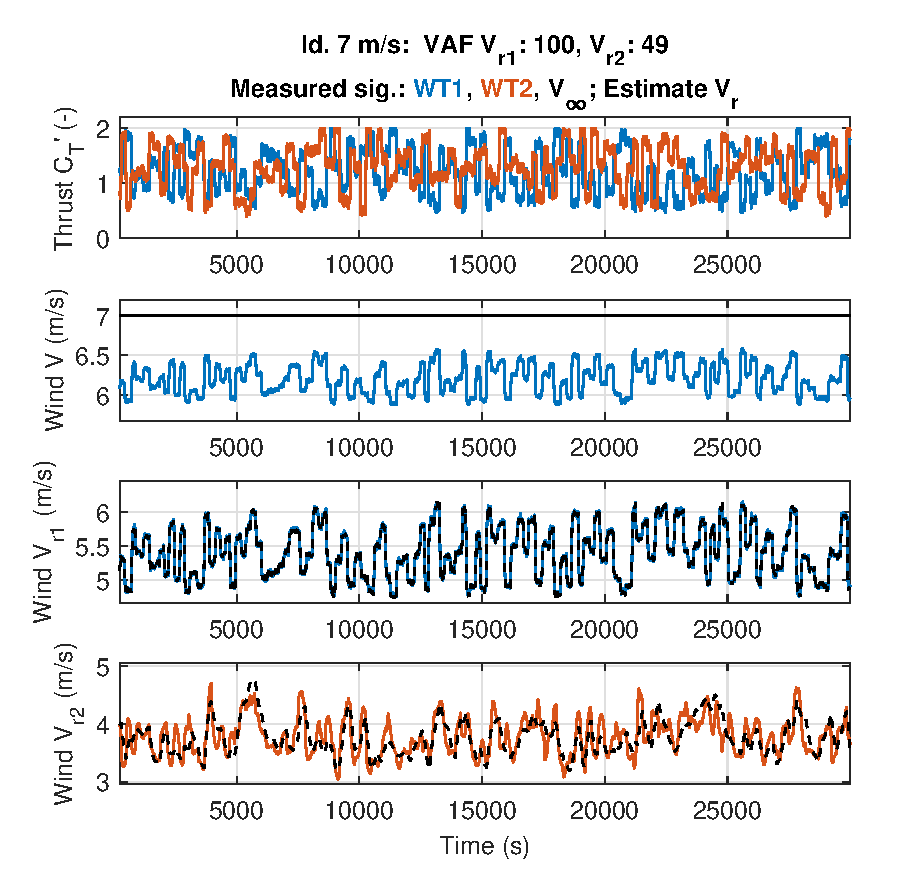
\includegraphics[width=0.485\textwidth]{figures/figures_CDC22/Fig00_AIC7mpers_OL_id.eps}}\hfill
 \subfloat[Verification dataset]{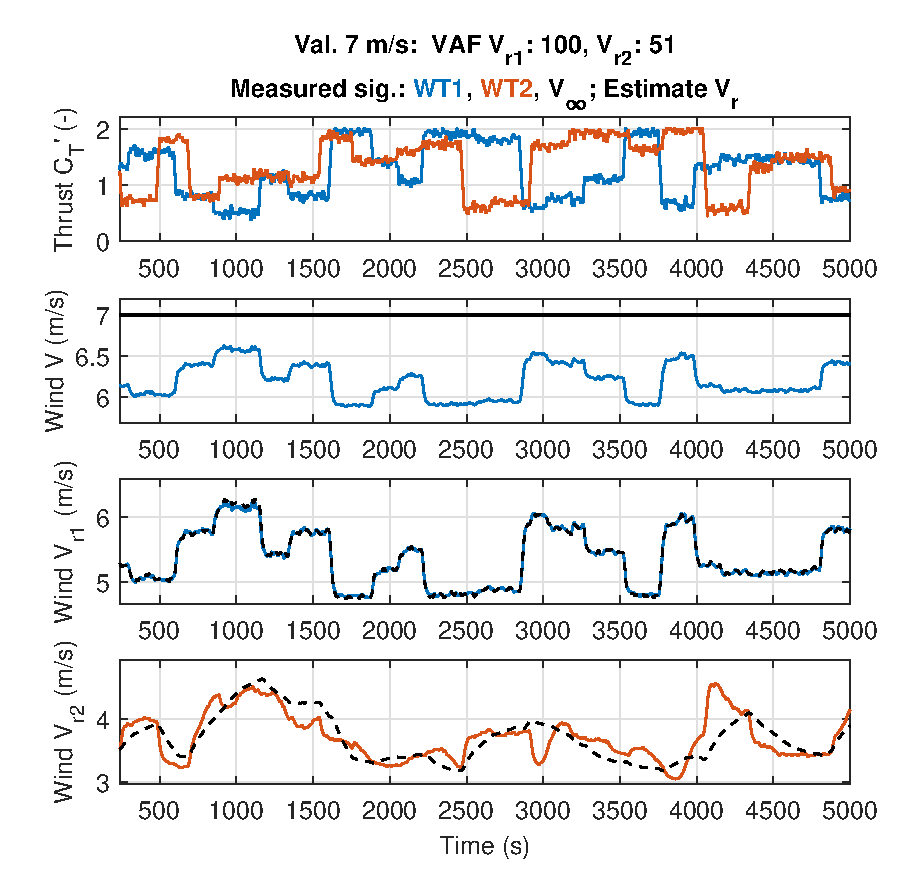
\includegraphics[width=0.485\textwidth]{figures/figures_CDC22/Fig00_AIC7mpers_OL_val.eps}}
     \caption[Identification and verification datasets at $V_\infty = 7$\,m/s for the Koopman model identification of the adaptive AIC algorithm]{Identification and verification datasets at $V_\infty = 7$\,m/s for the Koopman model identification of the adaptive AIC algorithm. Subplots (top to bottom): thrust $C_T^\prime$; constant wind speed $V_\infty$ (black) and $V_1$ (blue); real vs.estimated effective wind $V_{r1}, V_{r2}$. WT1/WT2 signals are blue/red; black dashed lines denote estimates.}
    \label{fig:IDdataAIC}
\end{figure}
To quantify the model's accuracy, the Variance Accounted For (VAF) is utilized to measure the similarity between the simulated and estimated effective wind speeds. This measure of how well the output signal variation is explained by the model is also used in previous studies on Koopman DMD, e.g., \cite{Cassamo.2020}, and is defined as:
\begin{equation}
    \text{VAF} = \max \left(0, \left( 1 - \frac{\operatorname{var}(\bm{X} - \hat{\bm{X}})}{\operatorname{var}(\bm{X})} \right) \right)  \cdot 100\%
\end{equation}
where $\bm{X}$ is the simulated or real signal, $\hat{\bm{X}}$ is the estimated signal, and $\operatorname{var}(\cdot)$ denotes the variance. 

It can be seen that these values are significantly different for the effective wind speed of the first turbine WT1. This turbine experiences constant freestream wind and its behavior can be predicted exactly by the change in its thrust control signal. The second turbine is much harder to predict, as it experiences wake from the second turbine. However, it can be seen that the VAF value is nearly the same between the identification and the verification dataset. 

A third dataset for with 9,999 samples is created with a step change of the freestream wind from 7\,m/s to 9\, m/s at the 5000th sample. A fourth one with $n_o = 29,999$ with a constant freestream wind spead of 9\,m/s, and the corresponding verification dataset with 9,999 samples. 

The offline-identified model, trained on the first dataset depicted in Figure~\ref{fig:IDdataAIC}(a), that is with constant wind speed of $7\,\mathrm{m/s}$, is validated against the dataset from the third simulation featuring a step change. As illustrated in Figure~\ref{fig:ValComp}(a), the offline-identified model fails to track the system states once the freestream wind speed deviates from the training condition. This discrepancy occurs because the Koopman operator identified at the lower wind speed cannot capture the altered aerodynamic sensitivity and wake dynamics present at the higher wind speed. However, with the adaptive AIC algorithm, the accuracies of the non-adaptive AIC algorithm under constant wind speed are nearly recovered for this more challenging test case. In \cite{sharan2022Koopman} VAF values between 86\% and 90\% were reported. With the updat

%\begin{figure}[ht]
%    \centering
%    \includegraphics[width=0.65\textwidth]{figures_CDC22/Fig01_OL_Update0_tex.eps}
%    \caption{Open-loop system identification validation using a non-adaptive Koopman model during a wind speed step change.}
%    \label{fig:Valoffline}
%\end{figure}

\begin{figure}[ht]
    \subfloat[Non-adaptive model ($V_\infty = 7$\,m/s)]{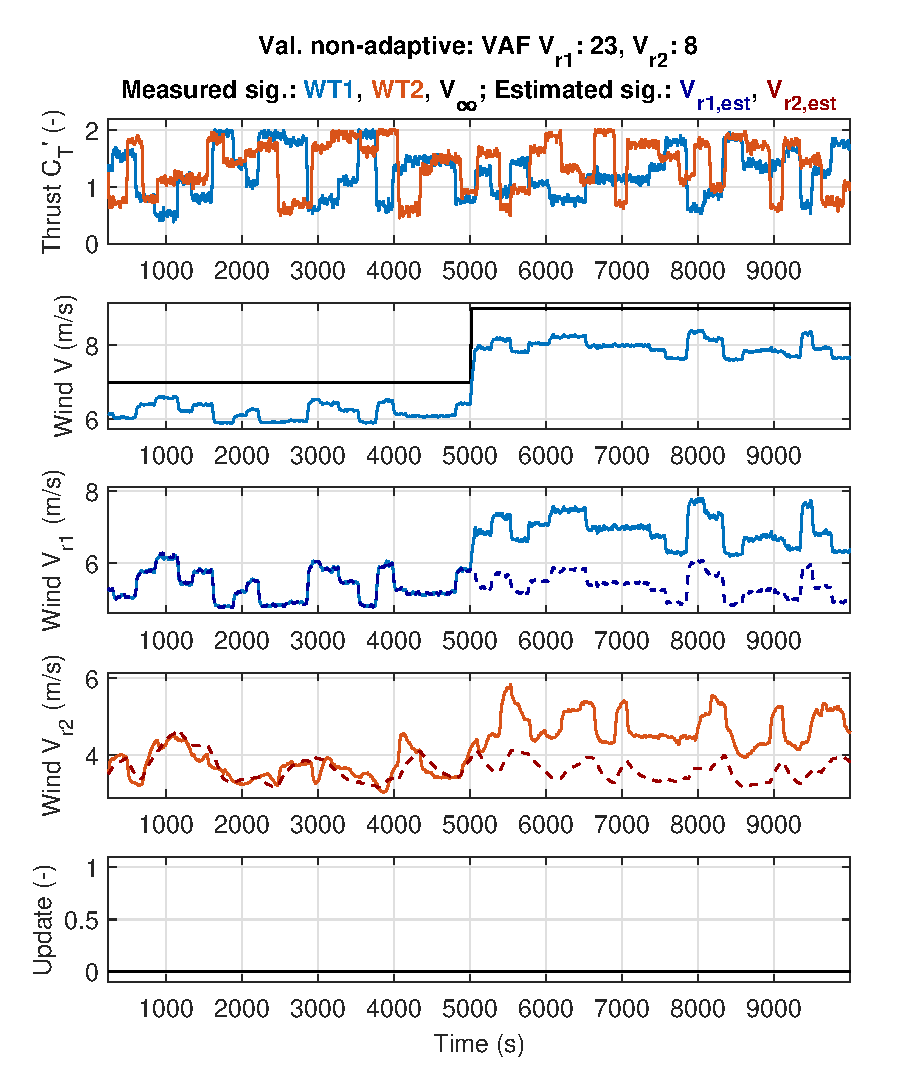
\includegraphics[width=0.485\textwidth]{figures/figures_CDC22/Fig01_OL_Update0_tex.eps}}\hfill
    \subfloat[Online-updated model]{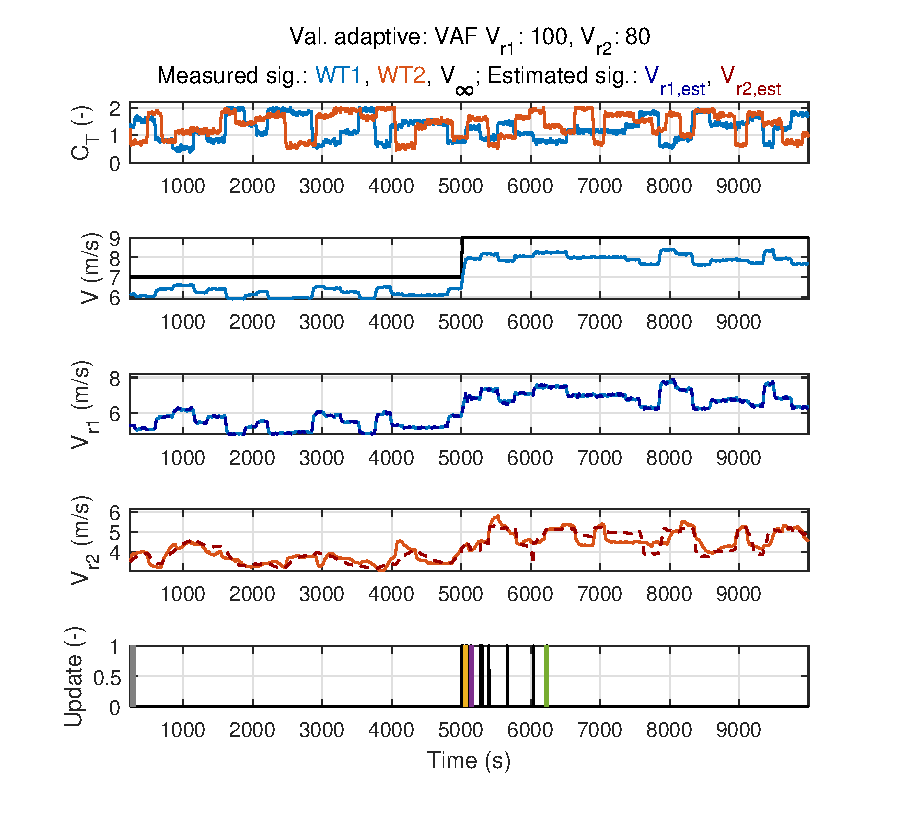
\includegraphics[width=0.485\textwidth]{figures/figures_CDC22/Fig02_OL_Update1_tex.eps}}
    \caption[Open-loop identification comparison during a wind speed step]{Open-loop identification comparison during a wind speed step at $t=5000$\,s. Subplots (top to bottom): thrust $C_T^\prime$; wind speeds $V_\infty$ (black) and $V_1$ (blue); real vs.estimated effective wind $V_{r1}, V_{r2}$; and the update signal (black). WT1/WT2 signals are blue/red; dashed lines denote estimates.}
    \label{fig:ValComp}
\end{figure}



The first subplot in Figure~\ref{fig:ValComp}(a) shows the thrust control signals (blue for Turbine WT1, red for Turbine WT2). The second plot shows the freestream wind speed in black and the wind measured directly in front of the first turbine in blue. The third and fourth plots display the simulated effective wind speeds as solid lines and the estimated values as dashed lines. Up to the wind speed change at $t = 5000\,\mathrm{s}$, the estimates follow the real data accurately. However, after the step, the model fails to predict the effective wind speed, resulting in a significant offset and an overall VAF of $0\%$ for both signals. In contrast, Figure~\ref{fig:ValComp}(b) presents the results from the online update scheme applied to the same dataset. With adaptation enabled, the estimated effective wind speeds $V_{r1}$ and $V_{r2}$ achieve VAFs of 99\% and 91\%, respectively. While the first four subplots display the same categories of signals as Figure~\ref{fig:ValComp}(a), the fifth subplot explicitly illustrates the update trigger logic. This plot indicates the instances where the model is updated because the discrepancy between the most recent five real and estimated data points exceeded the threshold $\nu$.

%\begin{figure}[ht]
%    \centering
%    \includegraphics[width=0.65\textwidth]{figures_CDC22/Fig02_OL_Update1_tex.eps}
%    \caption{Open-loop system identification using the online-updated Koopman model during a wind speed step change.}
%    \label{fig:Valonline}
%\end{figure}

Figure~\ref{fig:SingVal} depicts the maximum and minimum singular values of four linear Koopman models at different stages of the online update process. The black dashed line represents the result of a system identification performed offline using the complete dataset from the second open-loop simulation at 9\,m/s. The colored solid lines correspond to the singular values of specific update instances at sample index $k$, which are highlighted using matching colors in the fifth subplot of Figure~\ref{fig:ValComp}(b). The initial model (grey line) is calculated on the dataset of the first open-loop simulation that does not contain the wind speed step. Note that with a sampling interval of $t_k = 1$\,s, the index $k$ corresponds directly to the simulation time in seconds. Singular values represent the gain of a system over a frequency range, with the maximum and minimum singular values defining the bounds of the system's amplification of input signals. Investigating these trajectories allows for an assessment of how the identified dynamics evolve, as shifts in the singular values indicate that the model is successfully capturing the underlying system's frequency response under varying operating conditions.
\begin{figure}[ht]
    \centering
    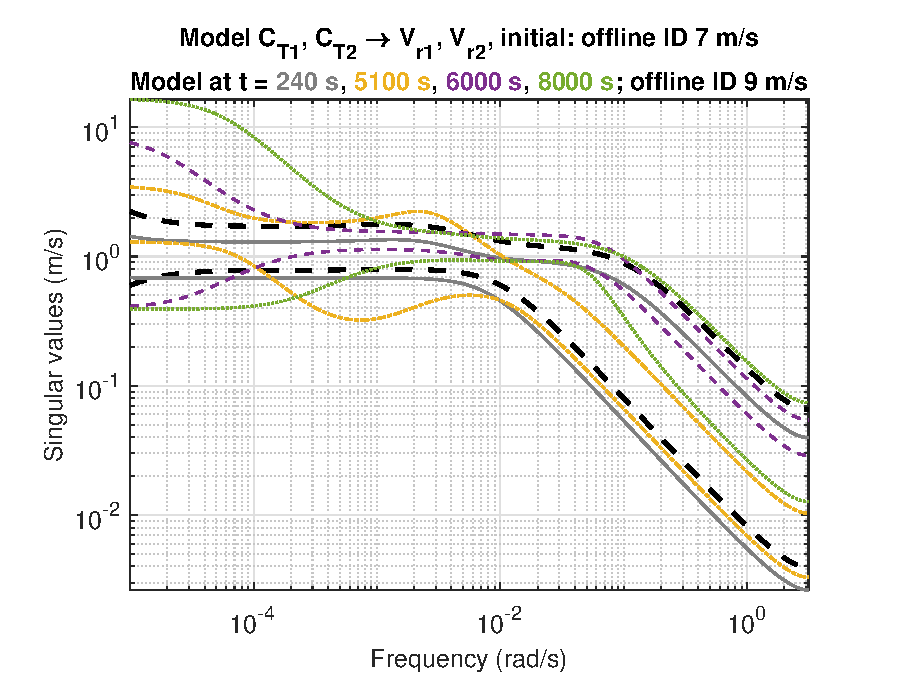
\includegraphics[width=0.65\textwidth]{figures/figures_CDC22/Fig03_OL_Bode_tex.eps}
    \caption[Maximum and minimum singular values of the Koopman models at various sample steps $k$ during online identification]{Maximum and minimum singular values of the Koopman models at various sample steps $k$ during online identification. The shift from the initial model (grey) to the final adapted model (green) demonstrates the convergence of the model's frequency response toward the reference offline identification (dashed black) following the wind speed step change.}
    \label{fig:SingVal}
\end{figure}

\begin{itemize}
    \item The grey line ($k = 240$) represents the initial Koopman model identified at $V_{\infty} = 7\,\mathrm{m/s}$. Its frequency response differs significantly from the reference offline model (black dashed line) identified with the fourth data set, obtained at $V_{\infty} = 9\,\mathrm{m/s}$ . 
    \item The yellow line ($k = 5100$) shows the model immediately after the wind speed step at $5000\,\mathrm{s}$. Following the wind speed step, the identification process uses data , causing the singular values to converge toward the low-pass behavior seen in the offline reference model. While the elevation in the low frequency range is still considerably visible in the red line, its decrease compared to the blue line indicates the adaptation to the new operating point.
    \item The purple line ($k = 6000$) illustrates the model during the transition as more data from the $9\,\mathrm{m/s}$ regime is incorporated.
    \item The green line ($k = 7949$) represents the final adapted model, showing a high degree of correlation with the reference offline model across the relevant frequency range. However,
\end{itemize}


The subsequent section presents closed-loop results obtained from WFSim using the adaptive Koopman model to provide effective wind speed estimates to the qLMPC controller. The value for the triggering condition $\nu$ was set to 0.15\,m/s which was found to be a good compromise between the number of updates and the accuracy of the estimation.

\subsubsection{Closed Loop Results}
A test case is implemented to demonstrate the benefits of the adaptive Koopman MPC algorithm versus the non-adaptive scheme. The simulation is run for $5000$\,s, resulting in a dataset of $5000$ samples. At sample $k = 2000$, the freestream wind $V_\infty$ increases from $7$\,m/s to $9$\,m/s with a ramp of $0.1$\,m/s per sample. The farm power reference $P_{\text{ref}}$ is increased in a step change from $1.72$\,MW to $2.58$\,MW at sample $k = 2500$. These values were selected to ensure the wind farm is physically capable of meeting the power demand at the given wind speeds.

The closed-loop performance is quantitatively evaluated using the Tracking Error (TE) and Actuator Activity (AA). While the Variance Accounted For (VAF) metric was previously used to validate the model's open-loop predictive accuracy, it is less suited for evaluating control success. In closed-loop operation, the primary objectives are to minimize the deviation from the power reference and reduce mechanical wear. Therefore, TE and AA are used as they directly correspond to the cost function terms minimized by the controller, as defined in Equation~\eqref{eq:NMPCcostAIC}. The specific weighting matrices $Q = 10^{-4}$ and $R = 10^{-6}$ used in the MPC cost function are the default values. They are used for all simulation shown in this thesis.

Figure~\ref{fig:CL_Comparison} compares the performance of the non-adaptive (a) and adaptive (b) Koopman MPC schemes.

\begin{figure}[ht]
    \centering
    % Subfigure (a): No online update
    \subfloat[Non-adaptive Koopman MPC] {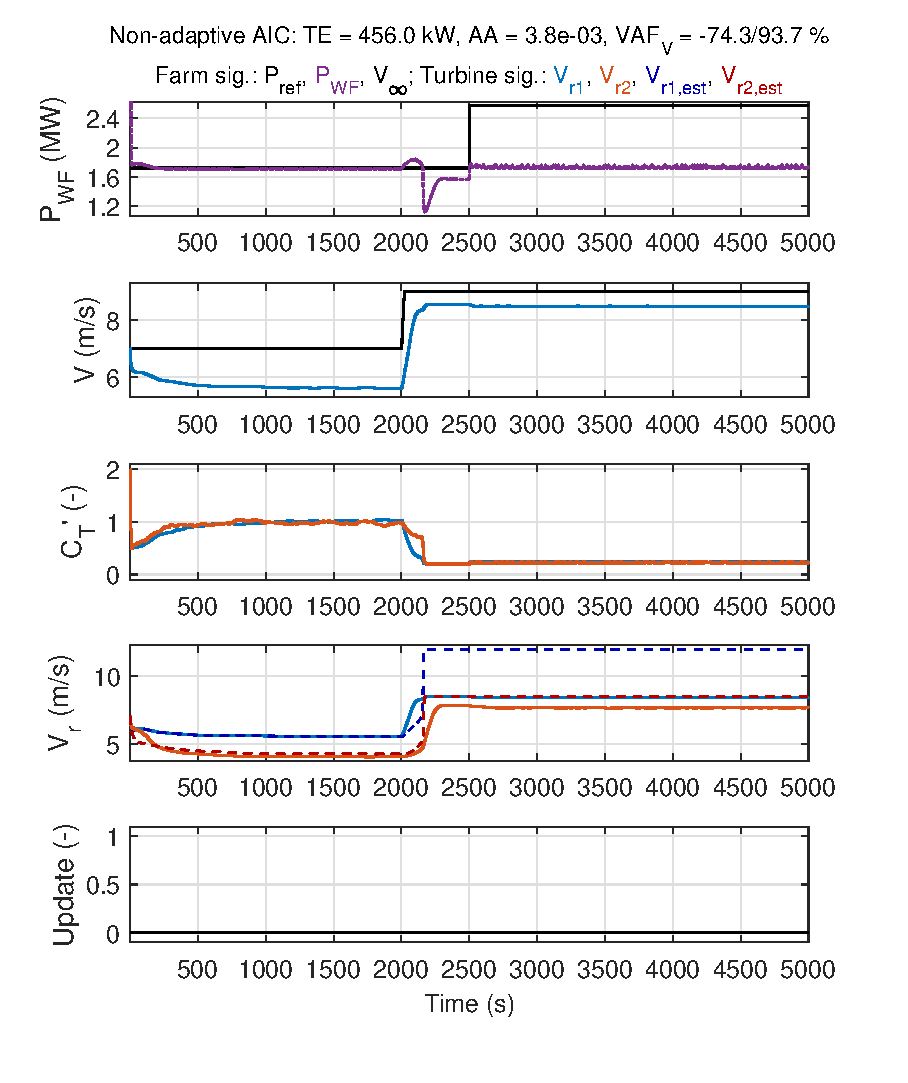
\includegraphics[width=0.495\textwidth]{figures/figures_CDC22/Fig04_CL_Update0_tex.eps}}\hfill
    \subfloat[Adaptive Koopman MPC with online updates]{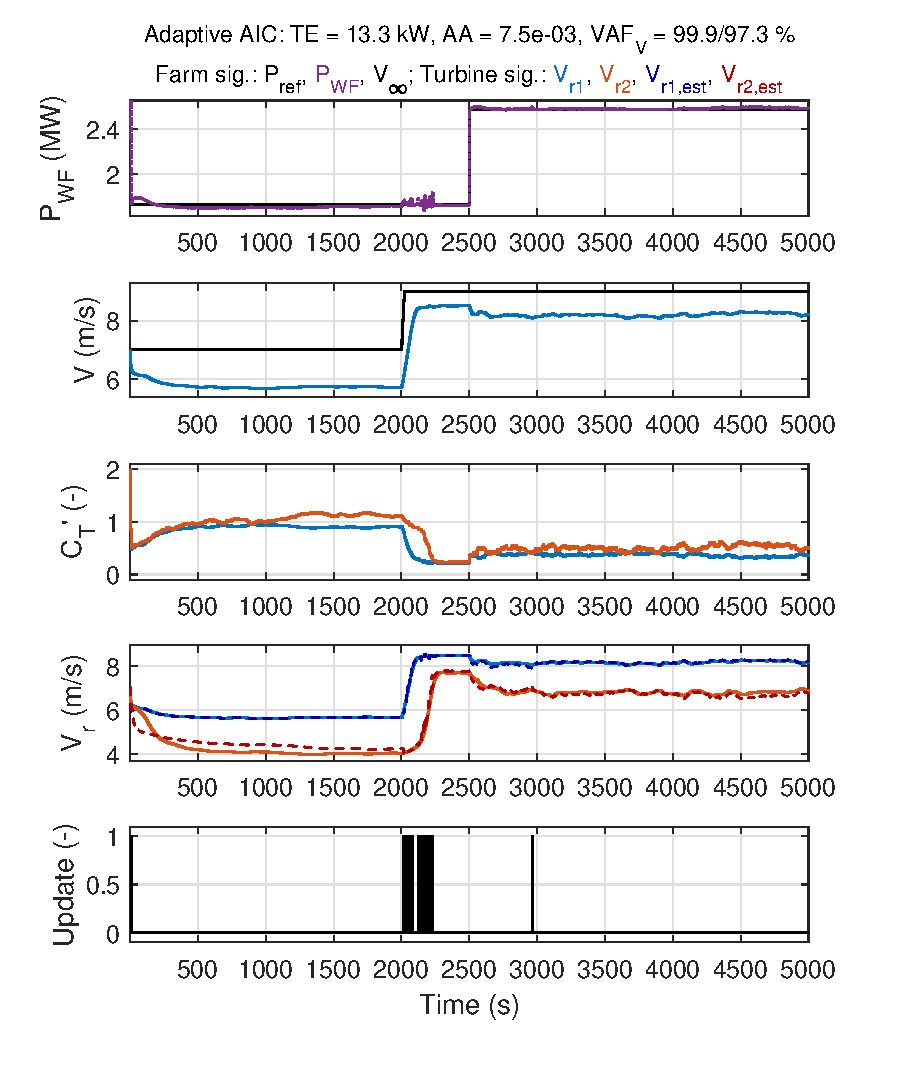
\includegraphics[width=0.495\textwidth]{figures/figures_CDC22/Fig05_CL_Update1_tex.eps}}
    \caption[Closed-loop tracking comparison during a wind speed ramp and power reference step.]{Closed-loop tracking comparison during a wind speed ramp and power reference step. Subplots (top to bottom): reference $P_{\text{ref}}$ (black) and farm power $P_{\text{WF}}$ (purple dashed); wind speeds $V_\infty$ (black) and $V_1$ (blue); thrust $C_T$; and real vs. estimated effective wind $V_{r1}, V_{r2}$. Bottom plot in (b) shows the update signal (black). WT1/WT2 signals are blue/red; dashed lines denote estimates.}
    \label{fig:CL_Comparison}
\end{figure}



The top subplots illustrate the farm-level power yield $P_{\text{WF}}$ (purple) relative to the reference signal $P_{\text{ref}}$ (black). The subsequent subplots display the freestream wind speed $V_{\infty}$ alongside the local wind speed $V_1$ measured at turbine WT1, followed by the thrust control inputs $C_{T1}$ and $C_{T2}$. Consistent with the previous identification plots, signals for WT1 are shown in blue and WT2 in red. The fourth and fifth rows compare the true effective wind speeds $V_{r1}, V_{r2}$ with their estimates, while the final subplot in Figure~\ref{fig:CL_Comparison}(b) indicates the specific instances where the Koopman model was updated online.

As shown in the first subplot of Figure~\ref{fig:CL_Comparison}(a), the non-adaptive scheme significantly overestimates the effective wind speeds following the transition. This leads to insufficient thrust coefficients $C_{T1}$ and $C_{T2}$, resulting in a large power tracking offset of $234.99$\,kW. In contrast, the online-updated model in Figure~\ref{fig:CL_Comparison}(b) reduces this offset to $14.52$\,kW. The adaptive scheme successfully tracks the effective wind speed despite changes in both the disturbance signal ($V_{\infty}$) and the power reference ($P_{\text{ref}}$).

However, a small increase in actuator activity is observed in the adaptive case. This is due to a persistent excitation signal added to the thrust coefficient to ensure the data remains informative for online identification. When the update condition is triggered, white noise is added to the control signal, updated every five samples. This augmented signal is a weighted sum of the optimal control input and the noise (weighted $0.99$ and $0.01$, respectively), ensuring that power tracking quality is maintained while satisfying the requirements for efficient online adaptation.

It should be noted that the precise and fast power tracking achieved by the adaptive Koopman MPC is partly attributable to the simplified turbine modeling in WFSim. The turbines are represented as actuator disks with a first-order filter on the thrust control signal, see Equation~\eqref{eqPowerWTAIC_vector}, while rotor inertia, drive-train and structural dynamics, and the turbine controllers are not modeled. In a higher-fidelity setup, the tracking response would likely be limited by mechanical time constants and structural load constraints. Therefore, while these results show the advantage of the adaptive over the non-adaptive Koopman approach, further validation with aeroelastic tools is necessary to assess the performance under realistic mechanical constraints.

The adaptive Koopman approach shows that effective wind speeds in waked wind farms can be predicted online with a data-driven model, provided that the operating conditions are similar to those covered by the training data. Since the model is only updated when the prediction error exceeds the threshold $\nu$, the computational effort remains low, while the prediction accuracy is maintained, with VAF values around 90\%  in both open- and closed-loop scenarios.In the closed-loop case, the adaptive strategy reduces the power tracking error by about 94\% compared to the non-adaptive scheme, at the cost of an increase in actuator activity of about 10\%. These results indicate that adaptive Koopman models are a suitable basis for wind farm control under varying freestream conditions. The following section builds upon this framework by integrating yaw control, exploring how WRC can be used alongside thrust control to further optimize total farm yield.



% This adaptive Koopman based approach for modelling highly
%nonlinear wakes hence estimates effective wind speed acting
%on wind turbines in a wind farm. An update rule is
%presented to enable online learning only when discrepancies between measurements and model estimates show that
%new measurements contain new information. Additionally,
%to provide sufficient information for the online update a
%small excitation test signal is superimposed on the control
%input if the update of the Koopman model is triggered. The
%WFSim environment was enhanced to support the use of
%changes in wind speed and used to generate test signals
%for open loop identification as well as a test environment
%for the designed controller. High VAF accuracies of wind
%estimations, around 90\%, were observed both in open and
%in closed loop. 
%In closed loop, the adaptive online-update strategy tracked the reference farm power well, outperforming recently presented non-adaptive schemes. Building on these promising results of applying adaptive Koopman models for wind farm control, possible future research directions are employing more realistic wind scenarios, including wind direction variations and the integration of yaw control. The next section discusses the inclusion of yaw control, as wake redirection control (WRC) represents a promising method to further increase overall wind farm yield.

\section{Wind Farm MPC with Combined Yaw and Thrust Control} 
\label{sec:WindFarmLinearMPCforWRC-AIC}

The control design presented in Section~\ref{sec:AdaptiveWindFarmqLMPCforAIC} is extended to include yaw control in addition to thrust control. Two data-driven WRC-AIC wind farm control approaches based on Koopman model predictive control are proposed and compared to a baseline AIC scheme. These WRC-AIC algorithms combine thrust and yaw control for power reference tracking and yield optimization:
\begin{enumerate}
    \item \textbf{Koopman wind estimation:}  
    The upstream turbine's yaw angle is computed to maximize power yield, while the thrust control signals of both turbines are determined via quasi-linear model predictive control (qLMPC) to minimize power tracking error and thrust variations. Both control actions are based on estimated effective wind speeds obtained from a Koopman model identified from open-loop WFSim data, using the control signals as inputs and the two effective wind speeds as outputs, as described in Section~\ref{sec:AdaptiveWindFarmqLMPCforAIC}.
    
    \item \textbf{Koopman farm power estimation:}  
    The upstream turbine's yaw angle and thrust coefficients are optimized simultaneously via linear MPC to minimize power tracking error as well as variations in thrust and yaw. In this case, the controller operates directly on the estimated total farm power, which is derived from a separate Koopman model identified with the same inputs as the first model but with the total wind farm power as the output.
\end{enumerate}
The first approach follows the concept introduced in \cite{boersma2017tutorial}. It verifies whether the power reference exceeds the so-called greedy power of the wind farm, defined as the power obtained when both turbines operate without yaw misalignment and at maximum thrust. If this condition is met, the yaw angle is gradually increased to an offline-calculated value that maximizes the overall wind farm yield. The second approach investigates whether smoother control signals can be achieved by jointly optimizing all available control inputs.

The test case corresponds to the same wind farm setup consisting of two turbines introduced in Section~\ref{sec:WindFarmSimulationWFSim} and used in Section~\ref{sec:AdaptiveWindFarmqLMPCforAIC}, with the wind direction aligned with the main axis of the farm. The two Koopman MPC designs leveraging combined WRC-AIC significantly reduce the tracking error compared to the previously presented baseline AIC algorithm. It is also demonstrated that this improvement can be achieved with relatively small yaw angles, thereby avoiding excessive mechanical loads on turbines operating with yaw misalignment. This makes the proposed approach a promising candidate for further investigation in three-dimensional medium- and high-fidelity simulation environments.

\subsection{Simulation Setup for Combined Yaw and Thrust Control} \label{WakeModel} 
As before, WFSim is used to obtain open-loop data and for closed-loop controller testing. This section provides an overview of the WFSim environment and describes the specific test cases utilized for Koopman system identification in this context.

Figure~\ref{fig:BlockDiagramFarm} illustrates the underlying concept for the WRC-AIC strategies applied to the two-turbine wind farm. Note that the primary difference from the setup in Section~\ref{sec:AdaptiveWindFarmqLMPCforAIC} is that the yaw control signal of the upstream turbine WT1, $\gamma_1$, is now an active control variable.

\begin{figure}[h]
    \centering
    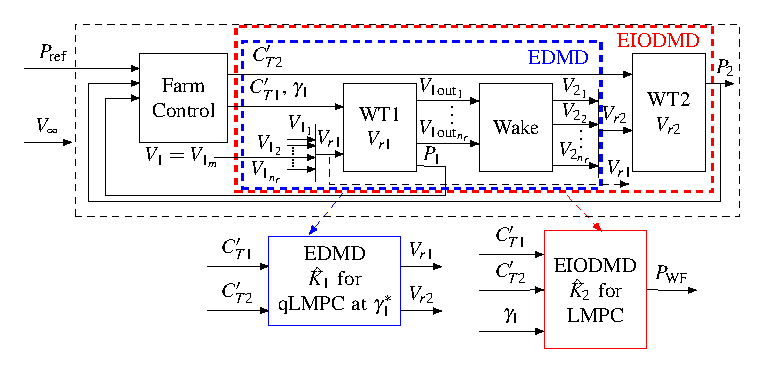
\includegraphics[width=0.9\textwidth]{figures/figuresBlockDiagram_IFAC23/farmCtrl17_P_multVthesis_WRCAIC_EIODMD.pdf}
    \caption[Block diagram of WFSim for WRC-AIC]{Block diagram of WFSim for WRC-AIC with farm control inputs $P_{\text{ref}}$, $P_1$, $P_2$, and $V_1 = V_{1_m}$, control signals $C_{T1}^{\prime}$, $C_{T2}^{\prime}$, $\gamma_1$, and freestream wind $V_\infty$. Local wind speeds upwind and downwind of WT1 are $V_{1_1} \dots V_{1_{n_r}}$ and $V_{1\text{out}_1} \dots V_{1\text{out}_{n_r}}$. Wind speeds upwind of WT2 are $V_{2_1} \dots V_{2_{n_r}}$. The input to the EDMD model (blue) are $V_1, C_{T1}^{\prime}, C_{T2}^{\prime}$ with effective wind outputs $V_{r1}, V_{r2}$. The input to the EIODMD model (red) are $V_1, C_{T1}^{\prime}, C_{T2}^{\prime}, \gamma_1$ with farm power output $P_{\text{WF}} = P_1 + P_2$.}
    \label{fig:BlockDiagramFarm}
\end{figure}

The signals are defined as in previous sections, with the exceptions that the freestream wind speed is kept constant and $\gamma_1$ is commanded by the farm controller. This results in the following signal configuration:
\begin{description}
    \item[-] The freestream wind $V_\infty$ is constant at $8$\,m/s and aligned perpendicular to the turbines for all simulations in this section.
    \item[-] The farm power reference $P_{\text{ref}}$.
    \item[-] The measured wind $V_1$ at WT1, used as a controller input as established in Section~\ref{sec:AdaptiveWindFarmqLMPCforAIC} and the underlying study~\cite{dittmer2022data}.
    \item[-] The thrust control signal $C_{T1}^{\prime}$ and yaw $\gamma_1$ of WT1, with the latter being a variable here, while it was fixed at $0$\,deg in Section~\ref{sec:AdaptiveWindFarmqLMPCforAIC}.
    \item[-] The effective wind speed $V_{r1}$ (mean wind speed over the rotor disk) and power $P_1$ of WT1.
    \item[-] Corresponding input and output signals for turbine WT2.
\end{description}
The farm layout and turbine parameters follow Table~\ref{table:WfSim}. For EDMD, estimates $\Tilde{U}_{ri}$ are calculated from $P_i$ assuming a known power coefficient $c_p$.

Previous publications utilizing WFSim~\cite{boersma2017tutorial,doekemeijer2018online, sharan2022Koopman, dittmer2022data} focused on thrust control $C_T^{\prime}$ for AIC, resulting in $n_u = n_{\text{WT}}$ control inputs. However, WFSim also supports yaw control $\gamma$ for wake redirection. In a two-turbine scenario, this could result in $2n_{\text{WT}}$ inputs; however, for this proof of concept, only the yaw of the first turbine is varied. Since the second turbine has no downstream neighbors, its optimal orientation remains $\gamma_2 = 0$\textdegree{}, resulting in $n_u = 3$ control inputs for this study.

Open-loop data is acquired from a WFSim simulation of $n_o = 28000$ samples, where one sample $k$ corresponds to $1$\,s. The thrust signals $C_{T1}^{\prime}$ and $C_{T2}^{\prime}$ are constructed from white noise (mean 1.7, variance 0.3, lower and upper limits 0.1 and 2.0, respectively) held constant for $5$\,samples. The yaw signal $\gamma_1$ is stepped by $5$\textdegree{} every $4000$\,samples from $0$\textdegree{} to $30$\textdegree{} and augmented with zero-mean band-limited noise (variance $0.5$\textdegree{}). These signals ensure data excitation across all relevant frequencies and control input combinations.

The matrices $\bm{X}_{\text{EIODMD}}$ and $\bm{X}_{\text{EIODMD},+}$ are constructed from input, state and output samples:
\begin{equation}
    \bm{w}(k) = \begin{bmatrix} C_{T1}'(k) \quad C_{T2}'(k) \quad \gamma_1(k) \end{bmatrix}^T, \quad \bm{x} = [V_{r1} \;\; V_{r2}]^T,  \quad 
    \bm{y}(k) = P_{\text{WF}}(k).
\end{equation}
and are assembled by stacking snapshots as follows:
\begin{align}
    \bm{X}_{\text{EIODMD}} &= \bigl[ [\bm{x}(k)^T \quad \bm{w}(k)^T]^T \bigr]_{k=1}^{n_o-1}, \\
    \bm{X}_{\text{EIODMD},+} &= \bigl[ [\bm{x}(k+1)^T \quad \bm{y}(k)^T]^T \bigr]_{k=1}^{n_o-1},
\end{align}
%
These matrices are used to construct two Koopman matrices, $\hat{K}_1 \mathbb{R}^{8\times8}$ (EDMD) and $\hat{K}_2 \in \mathbb{R}^{7\times9}$ (EIODMD), for the respective MPC designs. These matries are setup as follows: the system dynamics are of $6^{\text{th}}$ order with:
\begin{description}
    \item[-] Lifted states $\bm{\varphi} = [\bm{x}^T \;\; (\bm{x}^2)^T \;\; (\bm{x}^3)^T]^T$. As before, the quadratic and cubic terms reflect the relationship between wind, force and power.
    \item[-] Inputs $w_{K1} = [C_{T1} \;\; C_{T2}]^T$ and $w_{K2} = [C_{T1} \;\; C_{T2}'\;\; \gamma_1]^T$. Note that these vectors contained additionally the wind speed $V_1$ in \cite{dittmer2023koopman}.
    \item[-] EDMD outputs $\bm{y}_{K1} = [V_{r1} \;\; V_{r2}]^T$ and EIODMD outputs $\bm{y}_{K2} = P_{\text{WF}}$.
\end{description}
%
In \cite{dittmer2023koopman} the wind speed $V_1$ was part of the input vector and the following dimensions applied in that study: Matrix $\hat{K}_{w2} \in \mathbb{R}^{7\times10}$ is reordered to separate the contributions of the system states via the matrices $A_w \in \mathbb{R}^{6\times6}$ and $C_w \in \mathbb{R}^{1\times6}$, control inputs via $B_u \in \mathbb{R}^{6\times3}$ and $D_u \in \mathbb{R}^{1\times3}$, and the measured disturbance input $V_1$ via $B_d \in \mathbb{R}^{6\times1}$ and $D_d \in \mathbb{R}^{1\times1}$. To account for the disturbance as a state in the linear MPC, the matrices are augmented, resulting in the state-space matrices $A_{\hat{K}2} \in \mathbb{R}^{7\times7}$, $B_{\hat{K}2} \in \mathbb{R}^{7\times3}$, $C_{\hat{K}2} \in \mathbb{R}^{1\times7}$, and $D_{\hat{K}2} \in \mathbb{R}^{1\times3}$. The relationship to the original matrices obtained from EIODMD is given by:

\begin{align*} 
    \hat{K}_{w2} = \left[\begin{array}{c|cc} 
        A_w & B_d & B_u\\ 
        \hline 
        C_w & D_d & D_u 
    \end{array}\right] \implies
    \hat{K}_{2} = \left[\begin{array}{cc|c} 
        A_w & B_d & B_u\\ 
        \bm{0}_{n_d\times6} & \bm{I}_{n_d} & \bm{0}_{n_d\times3}\\
        \hline 
        C_w & D_d & D_u 
    \end{array}\right].
\end{align*}
with $n_d = 1$. In this study, without the wind speed $V_1$ as an input and hence with $n_d = 0$ and with $B_d$ and $D_d$ being therefore empty, there is

\begin{align*} 
    \hat{K}_{w2} = \left[\begin{array}{c|c} 
        A_w & B_u\\ 
        \hline 
        C_w & D_u 
    \end{array}\right] =
    \hat{K}_{2} \in \mathbb{R}^{7\times9},
\end{align*}
with the matrices $A_w$, $B = B_u$, $C_w$ amd $D_u$ having the dimensions as described above. 

The specific formulation and implementation of the qLMPC (based on $\hat{K}_1$) and linear Koopman MPC (based on $\hat{K}_2$) are detailed in Section~\ref{qLMPCDesign}.

%

%with state vector $\bm{x} = [V_{r1}\;\;V_{r2}]^T  $, input vector  $\bm{w} = [V_{r1}\;\;V_{r2}]^T  $
%The collected WFSim simulation signals are then used to calculate a Koopman matrix $\hat{K}_w$ via EIODMD,  as bases for the the MPC design. The system dynamics of the identified systems are of 6$^{th}$ order with 
%\begin{itemize}
%\begin{description}
%\item[-] inputs $w_{K1}$ as controls $C_{T1}^{\prime}$ and $C_{T2}^{\prime}$ and disturbance $V_1$, inputs $w_{K2}$ as all inputs $w_{K1}$ and additional control input $\gamma_1$
%\item[-] inputs $\bm{w}$ as control inputs $C_{T1}^{\prime}$, $C_{T2}^{\prime}$ and $\gamma_1$ and disturbance wind $V_1$,
%    \item[-] outputs of the EDMD wind estimation model as effective wind speeds, i.e. $y_{K1} = x = [V_{r1},V_{r2}]$
%\item[-] and outputs of the EIODMD power estimation model as farm power $y_{K2} = P_{\text{WF}} = P_1 + P_2$.
%\end{description}
%The values in the identified matrix $\hat{K}_w \in \mathbb{R}^{7\times10}$ are reordered to find the optimal three control inputs given measured wind $V_1$ and a power reference, both assumed constant over the prediction horizon. Hence, there is one additional disturbance state and three control inputs, resulting in augmented state $ \zeta_d = [\zeta^T  , V_1]^T   $ and matrices $\hat{K} \in \mathbb{R}^{8\times10}$, $A_{\hat{K}} \in \mathbb{R}^{7\times7}$, $B_{\hat{K}}\in \mathbb{R}^{7\times3}$, $C_{\hat{K}}\in\mathbb{R}^{1\times7}$, and $D_{\hat{K}}\in\mathbb{R}^{1\times3}$:


%$[\dot{x}_{K2},\dot V_1] = [A,B_d;0^{1\times7}] [x_{K2}, V_1]^T   + B_{K2} w $
%The matrix $Tilde(K)_2$, the result of the system identification with inputs $w_{K2}$ and output $$
\subsection{MPC Design for Combined Yaw and Thrust Control} \label{qLMPCDesign} 
Similar to the previously discussed AIC algorithm, the objective of the WRC-AIC wind farm controllers is to achieve accurate power reference tracking while minimizing changes in the control inputs. The WRC-AIC extends the previous approach by including the yaw of the first turbine as an additional control input, alongside the already used thrust control signals, which requires adjustments to the objective function and control algorithm. The main benefit of incorporating yaw, which is an increase in the achievable wind farm power output, will be demonstrated in the results presented in Section~\ref{SimResults}. In this section, the cost function to be optimized is defined, and the two MPC designs based on the Koopman matrices $\hat{K}_1$ and $\hat{K}_2$ are discussed.

The cost function $J(\bm{U})$ for both WRC-AIC schemes is formulated identically to the AIC algorithm, as given in Equation~\eqref{eq:errortraject}. It is based on the trajectories of the tracking error $\bm{E}$ and the changes in the control input $\Delta \bm{U}$:
\begin{align*} 
    J(\bm{U}) = \underbrace{\bm{E}^T \bm{Q} \bm{E}}_{J_Q (\bm{U})} + \underbrace{\Delta \bm{U}^T \bm{R} \Delta \bm{U}}_{J_R (\bm{U})},
\end{align*}
over a prediction horizon of $n_h$ sample steps. The weighting matrices are based on the scalar weights $Q$ and $R$, with the weight on the power error derived as $\bm{Q} = Q \bm{I}^{n_h \times n_h}$, as before. The weight on the control input changes is defined as
\begin{align*}
    \bm{R} = R \cdot \mathrm{diag}(R_{u1}, R_{u2}, \dots, R_{n_u}) \otimes \bm{I}^{n_h \times n_h},
\end{align*}
allowing differentiation of the penalty on changes in the different control inputs.

Correspondingly, the future error trajectory is $\bm{E}_k = \bm{P}_{\text{ref},k} - \bm{P}_{\text{WF},k}$, which is based on the total wind farm power. The change in control inputs is calculated as in Equation~\eqref{eq:UandDUAIC}.

For the two turbines considered and the default WFSim setting $n_h = 10$, the dimension of the control trajectory differs between the two approaches:
\begin{itemize}
    \item qLMPC approach ($\hat{K}_1$): The yaw angle $\gamma_1$ is optimized offline and kept as a static parameter during the control interval. Thus, only the two thrust signals are active control inputs, i.e., $n_u = 2$. This results in a trajectory $\Delta \bm{U}_{K1} \in \mathbb{R}^{20}$, as 2 inputs are optimized over 10 prediction trajectory steps.
    \item Linear MPC approach $\hat{K}_2$): The yaw angle $\gamma_1$ is included as a third active control input, resulting in $n_u = 3$. This yields a trajectory $\Delta \bm{U}_{K2} \in \mathbb{R}^{30}$ with 3 inputs set for 10 steps, with the control trajectory defined as:
    \begin{align*} 
        \bm{U}_{K2}(k) &= \begin{bmatrix} 
            C_{T1}^\prime(k) & C_{T2}^\prime(k) & \gamma_1(k) & \dots & \gamma_1(k+n_h-1) 
        \end{bmatrix}^T \in \mathbb{R}^{30 \times 1}.
    \end{align*}
\end{itemize}

For both designs, the cost function summands can be written as:
\begin{align*} 
    J_Q (\bm{U}) &= \big(\bm{P}_{\text{ref}} - (\tilde{\bm{L}} \bm{x}_0 + \tilde{\bm{S}} \bm{U})\big)^T \bm{Q} \big(\bm{P}_{\text{ref}} - (\tilde{\bm{L}} \bm{x}_0 + \tilde{\bm{S}} \bm{U})\big),\\
    J_R (\bm{U}) &= \Delta \bm{U}^T \bm{R} \Delta \bm{U},
\end{align*}
where the initial state $\bm{x}_0 \in \mathbb{R}^{3 n_T}$ is the state from the last sample, and the matrices $\tilde{\bm{L}} \in \mathbb{R}^{n_h \times 3 n_T}$ and $\tilde{\bm{S}} \in \mathbb{R}^{n_h \times n_h n_u}$ are used to calculate the expected future trajectory of the wind farm power $\bm{P}_{\text{WF}}$.

In the EDMD approach using $\hat{K}_1$, the original WFSim qLPV farm model is employed. The optimal yaw $\gamma_1^*$ is computed using the Gaussian wake model from~\cite{bastankhah2016experimental}, ensuring results are comparable to~\cite{boersma2019constrained}. The matrices $\tilde{\bm{L}}_{\hat{K}1}$ and $\tilde{\bm{S}}_{\hat{K}1}$ are calculated from $\bm{A}_{\text{WF}}$ and $\bm{B}_{\text{WF}}(\bm{V}_r)$.

In the EIODMD approach based on $\hat{K}_2$, the wind farm power $\bm{P}_{\text{WF}}$ is estimated directly. This results in a linear MPC, as effective wind speeds are no longer used as scheduling parameters. The stacked Toeplitz matrices $\bm{\Lambda}_{\hat{K}2}$ and $\bm{S}_{\hat{K}2}$ are constructed from the augmented matrices $\bm{A}_{\hat{K}2}, \bm{B}_{\hat{K}2}, \bm{C}_{\hat{K}2}, \bm{D}_{\hat{K}2}$ as:
\begin{align*}
    \bm{\Lambda}_{\hat{K}2} &= \begin{bmatrix}
        \bm{C}_{\hat{K}2} \\
        \bm{C}_{\hat{K}2} \bm{A}_{\hat{K}2} \\
        \vdots \\
        \bm{C}_{\hat{K}2} \bm{A}_{\hat{K}2}^{n_h-1}
    \end{bmatrix}, \quad
    \bm{S}_{\hat{K}2} =
    \begin{bmatrix}
        \bm{D}_{\hat{K}2} & \bm{0} & \dots & \bm{0}\\
        \bm{C}_{\hat{K}2} \bm{B}_{\hat{K}2} & \bm{D}_{\hat{K}2} & \dots & \bm{0}\\
        \vdots & \vdots & \ddots & \vdots \\
        \bm{C}_{\hat{K}2} \bm{A}_{\hat{K}2}^{n_h-2} \bm{B}_{\hat{K}2} & \dots & \dots & \bm{D}_{\hat{K}2}
    \end{bmatrix}.
\end{align*}
Since $\bm{P}_{\text{WF}}$ is the direct output of the EIODMD model, there is $\tilde{\bm{L}}_{\hat{K}2} = \bm{\Lambda}_{\hat{K}2}$ and $\tilde{\bm{S}}_{\hat{K}2} = \bm{S}_{\hat{K}2}$. Note that the inclusion of non-zero elements in the $\bm{D}_{\hat{K}2}$ matrix is a direct consequence of the simplified modeling approach used in WFSim. EIODMD is employed to map control signals directly to farm power without the intermediate scheduling parameter effective wind speed, which was used before. In this case, the relationship between the output power and thrust and yaw inputs is captured including a feedthrough term. This non-zero direct feedthrough reflects the absence of explicit turbine dynamics in the turbine power extraction model.

The next section presents simulation results obtained in WFSim both in open-loop and in closed-loop, using an AIC MPC as a baseline controller as well as the two WRC-AIC controller designs presented above.
%b_{KMPMC2,const} = [b_{const}, \delta u_M \mathbf{1}^{1\times N\cdotn_T}, -\delta u_m \mathbf{1}^{1\times N\cdot n_T}]^T  

%As the cost function is quadratic a reformulation of it as a QP problem gives a perfect reconstruction. Hence, we could show in \cite{adki2021MPC} that we get exactly the same results previously reported regarding power reference tracking performance in \cite{vali2019adjoint}, but with a 15 times speed-up.\\
%The accurate tracking performance is obtained in both \cite{vali2019adjoint} and \cite{adki2021MPC} by providing the effective wind speed of all turbines to the centralized farm controller. As mentioned previously, wind speeds might not be available for all wind turbines of a wind farm. In section \ref{SimResults} it is demonstrated that leveraging only wind estimated via the Koopman model good tracking performance can be achieved without wind measurements using a physically motivated identified model.
%The bounds of the first yaw angle, $u_{m,\gamma} = 0$ and $u_{M,\gamma} = 25$ are included in the vectors $u_m$ and $u_M$ that are used to form the input constraints $A_{c0,K2}$ and $B_{c0,K2}$, otherwise identically to $A_{c,K1}$ and $B_{c,K1}$.
%Moreover, the rate limits $\delta u$ of the rates are included via calculating the differences in rates with $\Delta_R$ with all values of the diagonal set to 1 and all values of the third supra-diagonal set to -1 to subtract the next value of the prediction horizon. In the current design $U^l$ is constant. Hence, the difference between the values of $\tilde{U}$ and $U$ is identical. Therefore, the new constraint matrices are: %for the MATLAB function \textit{quadprog} with linear constraints $A_{c} x < b_{c}$:
%\begin{align*} %\label{eqn:constraint}
%A_{c,K2} &= [ A_{c0,K2}, \Delta_R^T  , -\Delta_R^T  ]^T  \\
%B_{c,K2} &= [ B_{c0,K2},  \mathbf{1}^{1\times N\cdot n_T} \otimes (\delta u_M)^T  , \mathbf{1}^{1\times N\cdot n_T} \otimes (-\delta u_m)^T  ]^T  
%\end{align*}
%\begin{align*}
%[U,\Delta U]^T   - [u_M,u_{r,M}]^T   \le 0 \iff 
% [\tilde{U},\Delta_R \tilde{U}]^T   \le [-U^l,0]^T    + [u_M,u_{r,M}]^T    \\
%- [\tilde{U},\Delta_R \tilde{U}]^T   \le [U^l,0]^T    - [u_m,u_{r,m}]^T   %\\
% -U + u_m \le 0 \iff
%-\tilde{U} \le U^l  - u_m 
%\\&\iff -U\le -u_m 
%U- u_m \ge 0 -U-\left({-u}_M \right)\ge 0\\
% \end{align*}
%with rate limits $u_{r,M}$ and $u_{r,m}$ 

\subsection{Results} \label{SimResults}
Open-loop simulations are used to create signals that can be used to design the Koopman EDMD and IOEDMD models. Furthermore, an additional open loop simulation is run to investigate the potential power increase from WRC and to confirm the consistency between the results from the 2D NSE and the Gaussian wake model. Subsequently, closed-loop simulations are performed to evaluate power reference tracking performance.


\subsubsection{Open-Loop Results}
As in Section~\ref{sec:AdaptiveWindFarmqLMPCforAIC}, two datasets that differ from the one used for system identification in the original publication \cite{dittmer2023koopman} are designed. Both the identification dataset with $n_0 = 29,999$ samples and the verification data sets with 9.999 samples comprise combination of the two thrust controls and yaw control at different levels. 

 Figure~\ref{fig:WRCAICOL_EDMD} shows the results for the EDMD and the EIODMD identification. For the identification dataset, depicted in Figure~\ref{fig:WRCAICOL_EDMD}(a) and~(c), and for the verification dataset, presented in Figure~\ref{fig:WRCAICOL_EDMD}(b) and~(d), VAF values of more than 90\% are achieved for both datasets for the two effective wind speeds. 
\begin{figure}[htbp]
    \centering
    \subfloat[Identification dataset EDMD.]{
        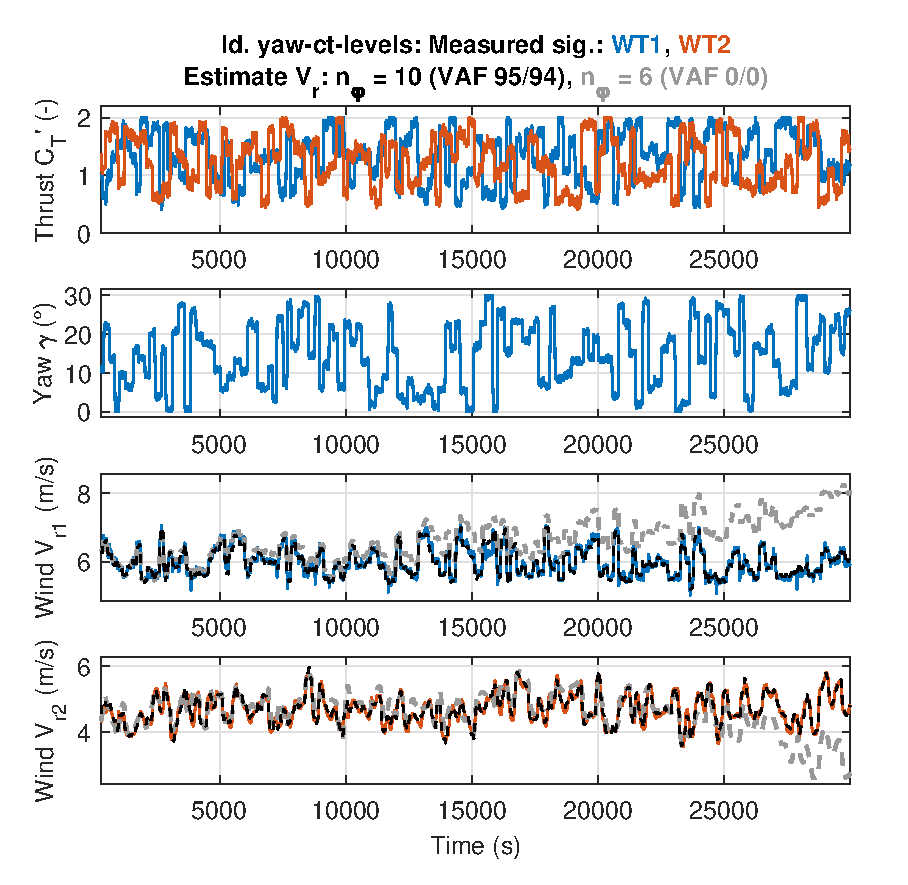
\includegraphics[width=0.485\textwidth]{figures/figures_IFAC23/03aFig_WRC_Id_Vr.eps}
        %\label{fig:WFSimgamma0}
    }
    \hfill
    \subfloat[Verification dataset EDMD.]{
        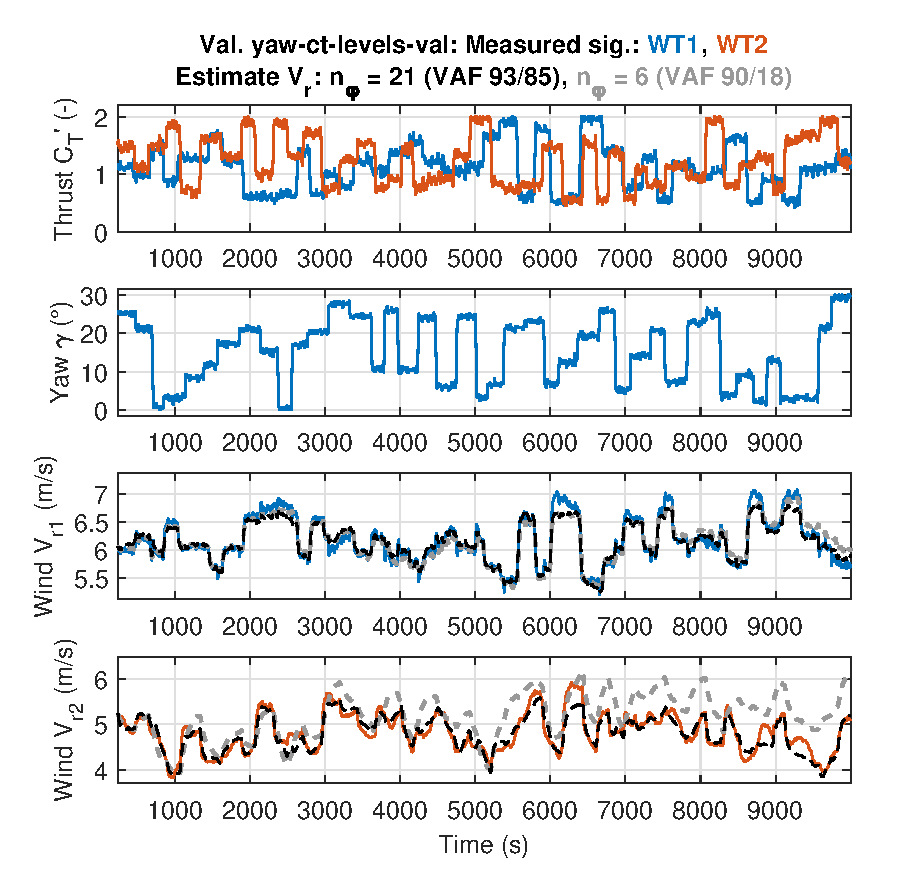
\includegraphics[width=0.485\textwidth]{figures/figures_IFAC23/03aFig_WRC_Val_Vr.eps}
       % \label{fig:PowerPerYaw}
    }\\
      \subfloat[Identification dataset EIODMD.]{
        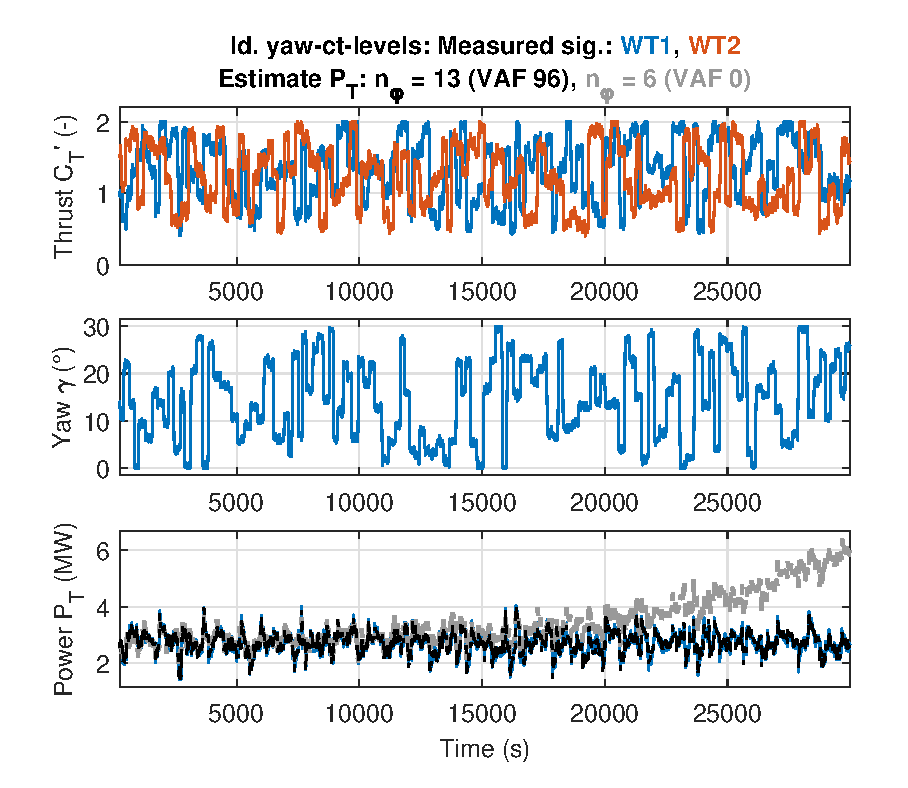
\includegraphics[width=0.485\textwidth]{figures/figures_IFAC23/03aFig_WRC_Id_P.eps}
        %\label{fig:WFSimgamma0}
    }
    \hfill
    \subfloat[Verification dataset  EIODMD.]{
        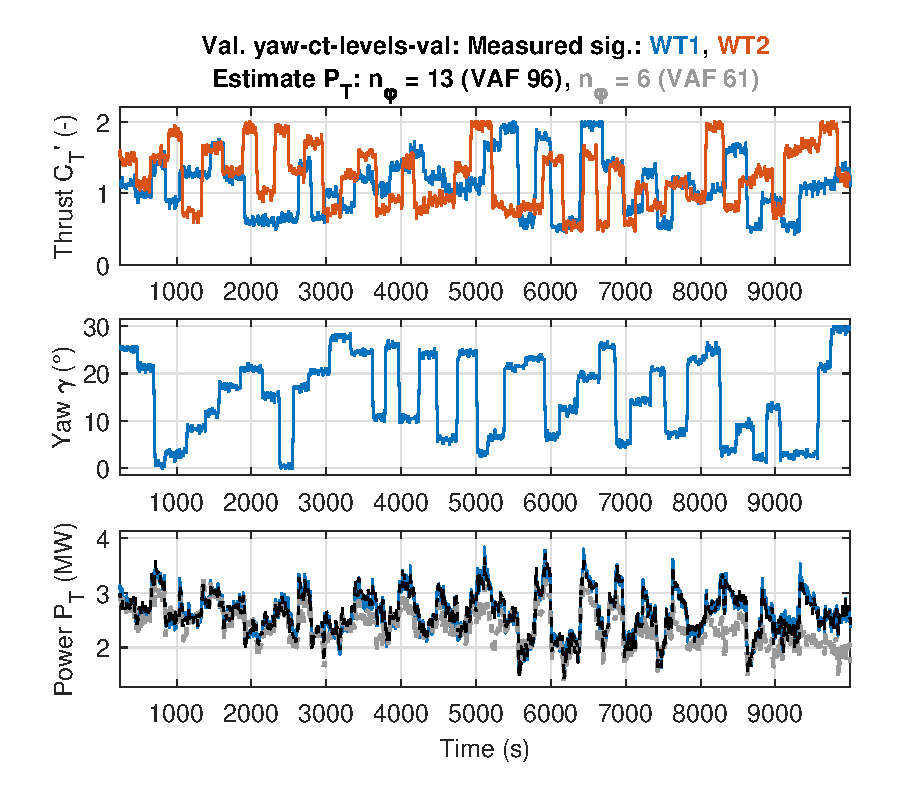
\includegraphics[width=0.485\textwidth]{figures/figures_IFAC23/03aFig_WRC_Val_P.eps}
        % \label{fig:PowerPerYaw}
    }
    \caption[Open-loop validation of the Gaussian wake model against WFSim.]{Identification and verification datasets for the Koopman matrices $\bm{\hat{K}}_1$ and  $\bm{\hat{K}}_1$. Subplots (top to bottom): Subplots (top to bottom): thrust $C_T^\prime$; constant wind speed $V_\infty$ (black) and $V_1$ (blue); real vs.estimated effective wind $V_{r1}, V_{r2}$. WT1/WT2 signals are blue/red; black dashed lines denote estimates.}
    \label{fig:WRCAICOL_EDMD}
\end{figure}


Apart from the above described datasets, open-loop WFSim simulation results to quantify the effect of wake misalignment are obtained for a step-sweep of the yaw angle $\gamma_1$ from 0\textdegree{} to 35\textdegree{} with consecutive increases of 5\textdegree{} every 500 samples, resulting in a total of 4000 samples. During this sweep, the thrust control signals are set to their maximum value of 2 and the freestream wind is held constant at 8\,m/s. Figure~\ref{fig:OpenLoopResultsCombined} shows the resulting longitudinal wind field and the power output of the turbines and farm.
\begin{figure}[htb]
\centering
\subfloat[Longitudinal wind field for $\gamma_1$ at 0\textdegree{} and 20\textdegree{}.]{
    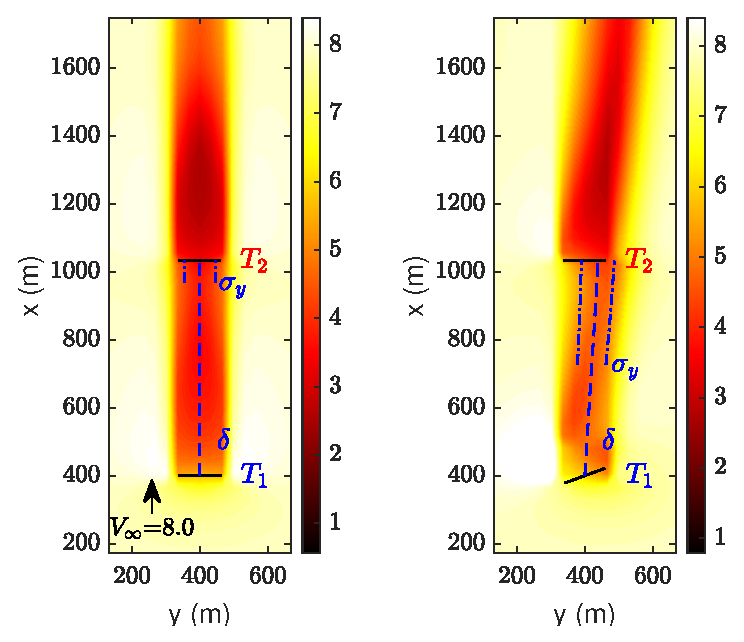
\includegraphics[width=0.48\textwidth]{figures/figures_IFAC23/03FigAngle0_20_tex.eps}
    \label{fig:WFSimgamma0}
}
\hfill
\subfloat[Power $P_{\text{WF}}$ as a function of yaw angle $\gamma_1$.]{
    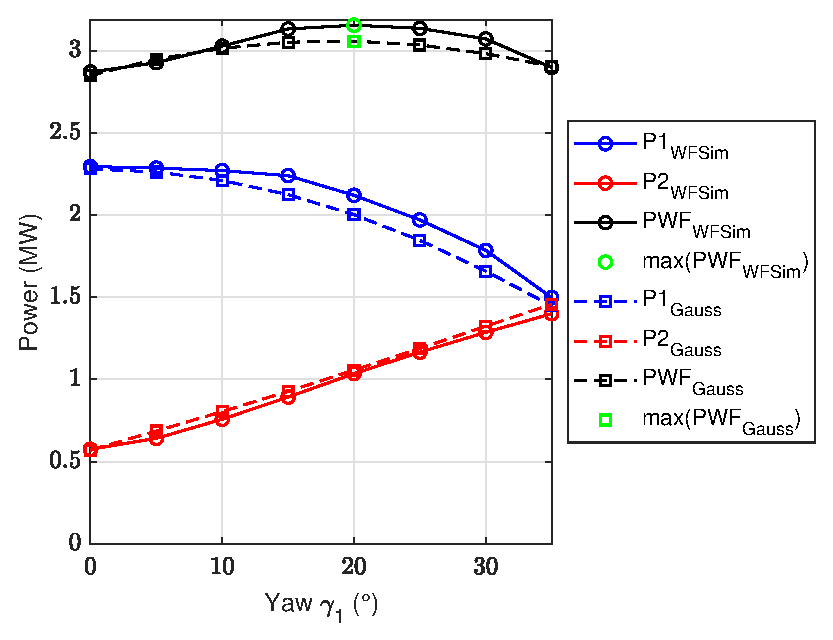
\includegraphics[width=0.48\textwidth]{figures/figures_IFAC23/01FigPwrVsYaw_tex.eps}
    \label{fig:PowerPerYaw}
}
\caption[Open-loop validation of the Gaussian wake model against WFSim.]{Open-loop validation of the Gaussian wake model against WFSim: (a) steady-state longitudinal wind field with Gaussian wake centerline $\delta$ and expansion $\sigma_y$ as blue dashed and dash-dotted lines; (b) power output comparison where WFSim results are marked with circles and the Gaussian model with squares: WT1 (blue), WT2 (red), total wind farm (black), and maximum power point (green)}
\label{fig:OpenLoopResultsCombined}
\end{figure}

Figure~\ref{fig:WFSimgamma0} visualizes the simulated longitudinal wind in steady state. The WFSim results, obtained by solving the 2D NSE \cite{boersma2018control}, are overlaid with the Gaussian wake model from \cite{bastankhah2016experimental}, with the centerline plotted as a blue dashed line and the far-field wake expansion as a blue dash-dotted line. The match of the wake expansion at the downstream rotor is reasonable. While the deflection angle of the Gaussian wake model in the far-wake region is slightly smaller than that of WFSim, the main area of speed deficit is nearly identical between the two. It should be noted that the wake centerline of a yawed turbine is curled in the near-wake region; therefore, modeling the centerline as a straight line in this region necessarily leads to discrepancies. This effect is addressed in more recent models such as the curled wake model \cite{martinez2019aerodynamics} or the Gaussian-Curl-Hybrid model \cite{king2020controls}, which have been shown to yield a better fit to large-eddy simulations and also report that the Gaussian model underestimates the power gain from wake steering. The standard Gaussian wake model is nevertheless used here for its simplicity, as it provides the optimal yaw angle with negligible computational effort.

Figure~\ref{fig:PowerPerYaw} shows the steady-state power at the end of each yaw step as a function of the yaw angle $\gamma_1$ for both WFSim and the Gaussian wake model. The power of the upstream turbine (blue) decreases as the yaw angle increases. This reduction is attributed to the reduced effective rotor area facing the wind and the inherent decrease in aerodynamic efficiency during yawed operation. These effects are analyzed in a comparative study of various yaw models \cite{sant2016comparing} and are further supported by recent field evaluations \cite{hulsman2022turbine}. Between 10\textdegree{} and 30\textdegree{}, the WFSim power of the first turbine slightly exceeds the Gaussian wake model prediction.

At farm level, the power increase due to WRC is 10\% in WFSim, compared to 6\% predicted by the Gaussian model. While this difference is non-negligible, the curves remain in close agreement, and both models identify the maximum farm power (green marker) at approximately 20\textdegree{} yaw, within the 5\textdegree{} resolution of the sweep. The matching location of the maximum and the similar curve shapes indicate that the Gaussian wake model is a computationally efficient and reasonable approximation of WFSim for determining the yaw angle in the combined controller, while the effective wind speeds for the thrust control are predicted with the Koopman model.

%\cite{boersma2019constrained}
% the deduction from the simulated wind fields

\subsubsection{Closed-Loop Results}
Figure~\ref{fig:ClosedLoopComparison} compares the closed-loop performance of the baseline AIC controller with the two WRC-AIC designs from Section~\ref{qLMPCDesign}, which combine yaw and thrust control.
\begin{figure}[!tbp]
\centering
\subfloat[Baseline AIC ($n_u = 2$) with fixed yaw ($\gamma_1 = 0^\circ$).]{
    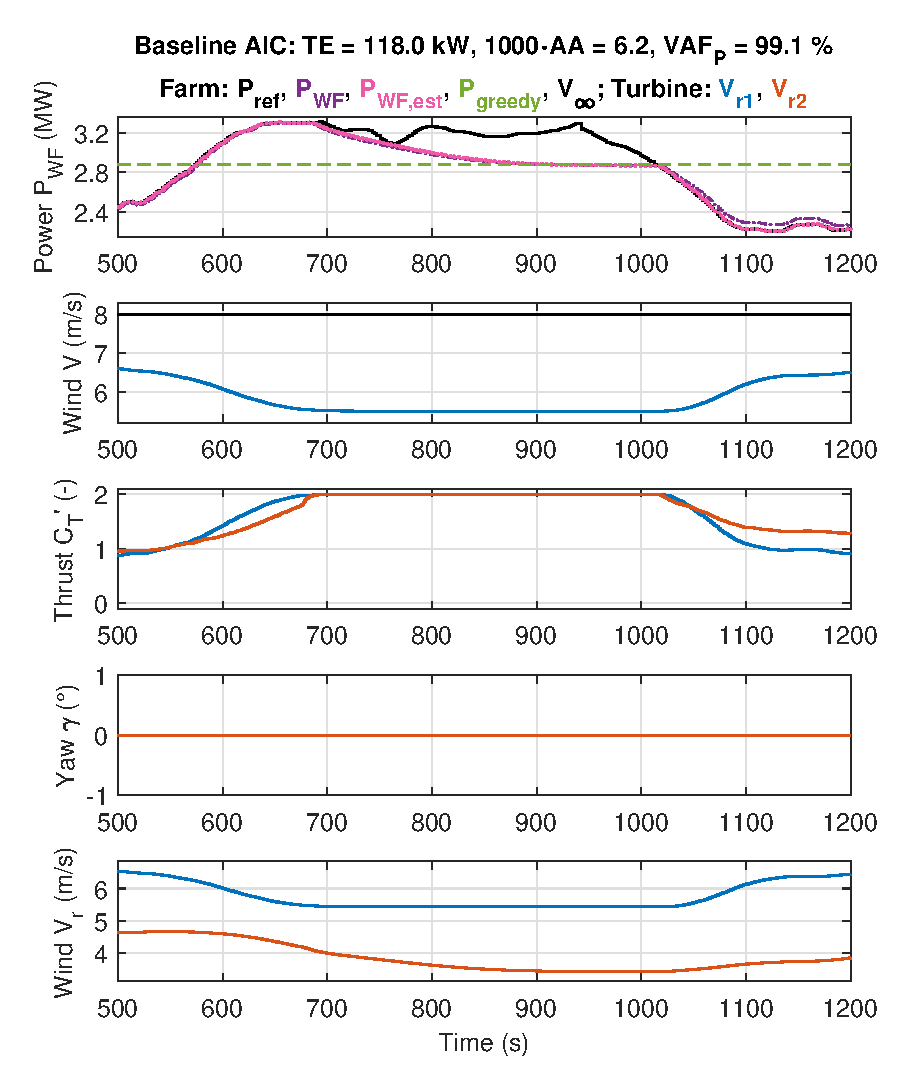
\includegraphics[width=0.48\textwidth]{figures/figures_IFAC23/04FigTimeSeries0_tex.eps}
    \label{fig:CLbaseline}
}
\hfill
\subfloat[AIC ($n_u=2$) with yaw set to the Gaussian-model optimum $\gamma_1^* = 18^\circ$ when $P_{\text{ref}} > P_{\text{greedy}}$.]{
    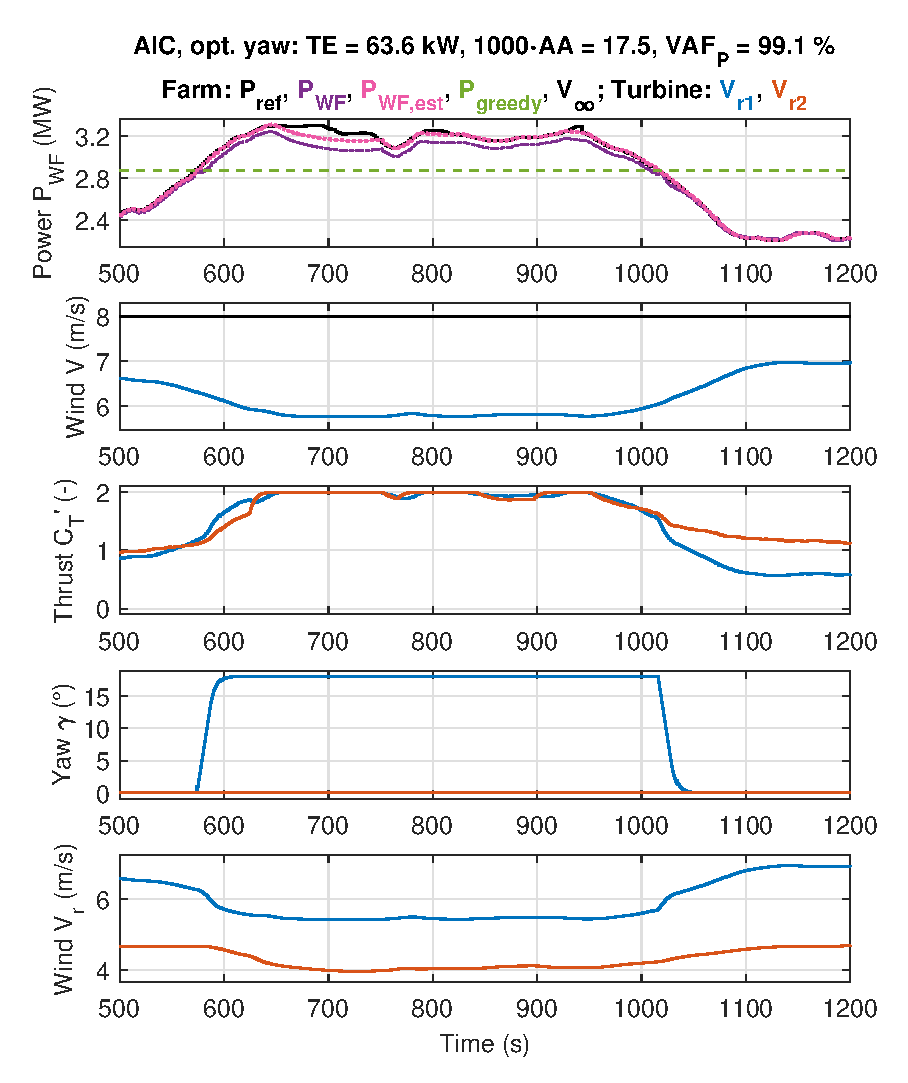
\includegraphics[width=0.48\textwidth]{figures/figures_IFAC23/05FigTimeSeriesQLMPC_tex.eps}
    \label{fig:CLMPC1}
}

\vspace{0.5cm}

\subfloat[WRC-AIC ($n_u=3$): thrust and yaw controls optimized simultaneously.]{
    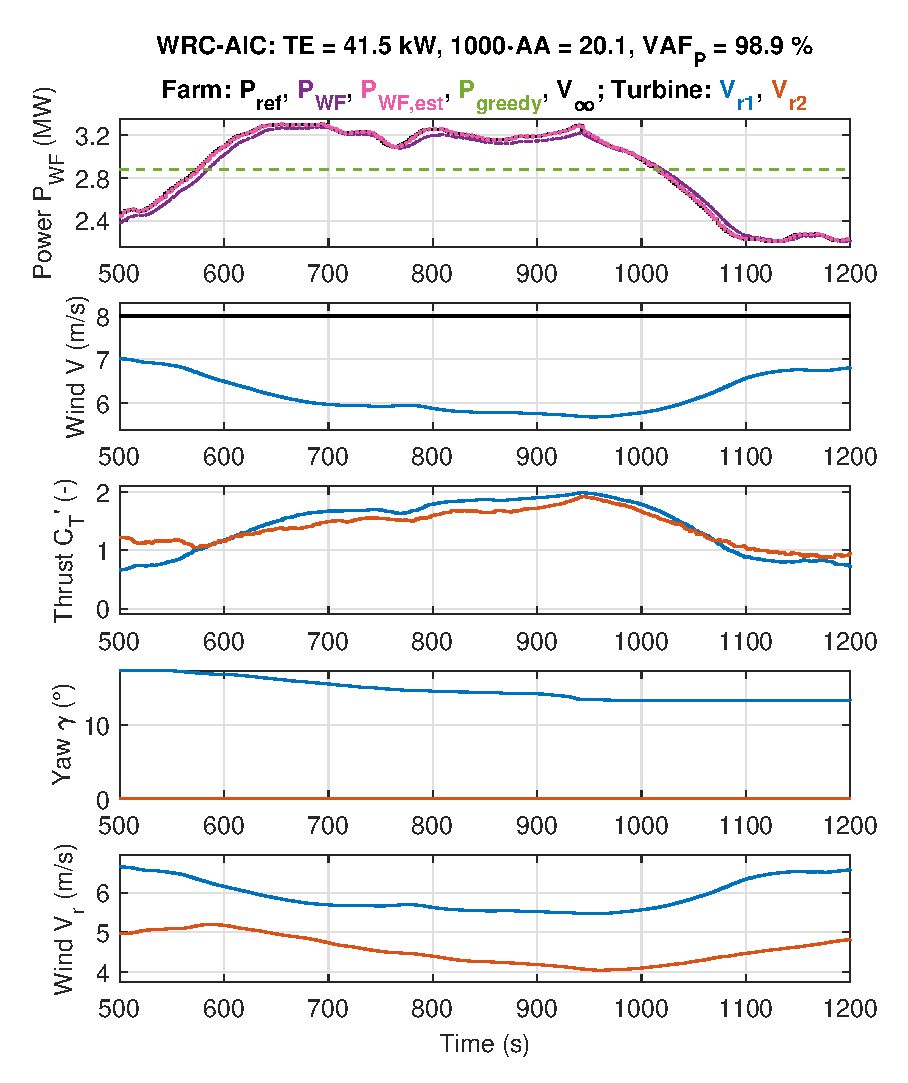
\includegraphics[width=0.48\textwidth]{figures/figures_IFAC23/06FigTimeSeriesLinMPC_tex.eps}
    \label{fig:CLMPC2}
}

\caption[Closed-loop performance comparison of the baseline AIC and the two WRC-AIC algorithms]{Closed-loop performance comparison of the baseline AIC and the two WRC-AIC algorithms. Subplots (top to bottom): reference $P_{\text{ref}}$ (solid black), farm power $P_{\text{WF}}$ (purple dashed), and greedy power $P_{\text{greedy}}$ (green dashed); wind speeds $V_\infty$ (black) and $V_1$ (blue); thrust $C'_T$; yaw $\gamma$; and real vs. estimated effective wind speeds $V_{r1}, V_{r2}$. WT1/WT2 signals are blue/red; dashed lines denote estimates.}
\label{fig:ClosedLoopComparison}
\end{figure}
The controllers are tasked with tracking a dynamic power reference signal, defined as:
\begin{align*}
P_{\text{ref},k} = \big(a_{\text{const}} + a_{\delta} \, \delta P_k \big) P_{\text{greedy}},
\end{align*}
where $\delta P_k$ is a random sequence as in \cite{sharan2022Koopman}, and $P_{\text{greedy}}$ represents the maximum power production of the farm when both turbines operate at maximum thrust ($C_T' = 2$) and zero yaw ($\gamma = 0^\circ$). While the original parameters in \cite{sharan2022Koopman} were set to $a_{\text{const}} = 0.8$ and $a_{\delta} = 0.35$, the present work uses $a_{\text{const}} = 0.9$ and $a_{\delta} = 0.2$, and the vector $\delta P$ has been resampled to update only every second time step. These modifications yield a reference trajectory that exceeds the greedy power for longer durations, thereby increasing the importance of wake steering for successful tracking. To ensure that the performance metrics are not affected by initialization artifacts, the evaluation begins at sample $k=240$.

The closed-loop performance is evaluated using the tracking error (TE) and actuator activity (AA) metrics introduced in Section~\ref{section:AICWindFarmControl}. These metrics correspond to the weighted terms of the cost function in Equation~\eqref{eq:NMPCcostAIC}, where the scalar weights $Q$ and $R$ are given in the subplot titles of Figure~\ref{fig:ClosedLoopComparison}. For the combined control case, the input-specific weighting factors are set to $R_{u1} = R_{u2} = 1$ for the thrust control increments $\Delta C_{T1}^\prime$ and $\Delta C_{T2}^\prime$, and $R_{u3} = 0.1$ for the yaw increment $\Delta \gamma_1$. Both TE and AA are computed as mean values over the evaluation period, with the AA including the respective weighting factors.

Figure~\ref{fig:CLbaseline} shows the performance of the baseline controller with the yaw angle fixed at zero. Figure~\ref{fig:CLMPC1} shows the results of the first Koopman MPC algorithm ($n_u=2$), based on an EDMD model, which sets the yaw angle to the optimum of the Gaussian wake model whenever the reference exceeds the greedy power. Here, $\gamma_1^* = 18^\circ$ is the exact optimum of the Gaussian model, while the open-loop sweep in Figure~\ref{fig:PowerPerYaw} resolves the maximum only to 5\textdegree{}. Finally, Figure~\ref{fig:CLMPC2} shows the results of the second Koopman MPC algorithm ($n_u=3$), based on an EIODMD model, which optimizes thrust and yaw simultaneously. The first plot in each subfigure shows the wind farm power $P_{\text{WF}}$, the power reference $P_{\text{ref}}$, and the greedy power $P_{\text{greedy}}$.

In Figure~\ref{fig:CLbaseline}, with the thrust coefficient as the only actuator, the farm power initially exceeds the greedy power when the reference demands it. However, it falls back to the greedy power once the increased wind speed deficit from the first turbine's higher thrust reaches the second turbine. In Figure~\ref{fig:CLMPC1}, the yaw angle is increased when the reference exceeds the greedy power, which reduces the tracking error by a factor of 1.8.

In Figure~\ref{fig:CLMPC2}, the tracking error is further reduced from 116\,kW to 33\,kW by including the yaw angle as a third control input. The actuator activity increases slightly compared to the EDMD design, as the yaw angle changes more frequently. However, the EIODMD-based controller results in both smaller thrust coefficients and smaller yaw angles. This is desirable, as it is expected to reduce the loads acting on the tower and blades.

These results show that the Koopman-based WRC-AIC MPC effectively coordinates yaw and thrust to overcome the wake-induced limitations of AIC alone. The following section concludes the chapter by summarizing the key results and discussing the limitations and future research directions for Koopman-based wind farm control.


\section{Conclusions}
This chapter presented and analyzed three applications of DMD using Koopman lifted functions
for wind farm control. The first part discussed the modifications required in the WFSim simulation
environment to enable adaptive control testing and to investigate the influence of intentional yaw
misalignment through a yaw-angle-dependent power coefficient. This was followed by the design,
implementation, and evaluation of an adaptive AIC controller, and subsequently, two WRC-AIC
controllers combining wake redirection and axial induction control.

Table~\ref{tab:WindFarmSummary} summarizes the quantitative evaluation criteria of the
closed-loop simulation runs. The focus of this study was to improve the tracking error, i.e., the
mean difference between the grid demand and the farm power output. The weighted square of
this error is also the first summand of the MPC optimization function. However, the weighting
function also contained the weighted square of the actuator rate. As the original weights from
the simulation environment were not changed, the actuator rate penalty was small relative to
the tracking error weight, allowing rapid thrust changes without penalizing actuator activity.
This results in an increase in actuator activity, i.e., the thrust rate of the rotors increases,
which is most pronounced in the WRC-AIC case. Future research might look into finding a
more balanced approach between decreasing tracking error and limiting actuator activity.

\begin{table}[h]
\centering
\caption[Wind farm controller evaluation criteria: Tracking error and
actuator activity for adaptive AIC (wind speed change) and AIC vs two WRC schemes (challenging power reference).]{Wind farm controller evaluation criteria.
    Tracking error (TE) and actuator activity (AA) for the adaptive AIC
    ( Section~\ref{sec:AdaptiveWindFarmqLMPCforAIC}, wind speed change $V_\infty = 7$--$9$\,m/s)
    and the WRC-AIC algorithms
    (Section~\ref{sec:WindFarmLinearMPCforWRC-AIC}, challenging power reference $V_\infty = 8$\,m/s).
    Results are not directly comparable across sections due to different
    test cases ($Q = 10^{-4}$, $R = 10^{-6}$).}
\label{tab:WindFarmSummary}
\begin{tabular}{ll rr}
    \toprule
    Section & Controller & TE (kW) & $\text{AA} / 10^{-3}$\,(-) \\
    \midrule
    \multirow{2}{*}{AIC}
    & Baseline, non-adaptive AIC  & 234.99 & $2.06$ \\
    & Adaptive AIC                &  14.52 & $2.27$ \\
    \midrule
    \multirow{3}{*}{WRC-AIC}
    & Baseline AIC ($\gamma_1 = 0^\circ$)              & 123.24 & $6.69$ \\
    & AIC + Gaussian yaw ($\gamma_1^* = 18^\circ$)     &  75.24 & $13.1$ \\
    & WRC-AIC EIODMD ($n_u = 3$)                       &  32.73 & $15.6$ \\
    \bottomrule
\end{tabular}
\end{table}

The results highlight several important findings. Physics-informed lifting functions were shown
to effectively capture both the relationship between control inputs and effective wind speeds and
the mapping from control inputs to power outputs. Furthermore, it was demonstrated that
Koopman-based estimation models can be updated online in real time, enabling adaptive control
under non-stationary wind conditions. The inclusion of WRC led to a notable increase in total
farm power output---exceeding 5\%. Specifically, the Bastankhah analytical wake model predicted
an improvement of approximately 6\%, while the WFSim simulation indicated an increase of
around 10\%. These results are consistent with trends reported in related literature. Both the
Bastankhah and the Navier--Stokes-equation-based WFSim models showed good agreement in
terms of wake expansion and power prediction. The combination of increased power yield and
precise model representation resulted in accurate power reference tracking, even for reference
signals exceeding the greedy power. This outcome underscores the potential of Koopman-based
WRC-AIC control strategies to enhance wind farm efficiency and support grid stability through power delivery more closely following the demanded power.

